\section{存储管理}

\begin{frame}[fragile]{新问题}
  \begin{easylist}  \easyitem
    & 通过进程管理,OS可以控制管理程序的运行,并通过处理机调度,决定要哪一个程序
    运行。
    & 现代计算机的体系架构要求程序要读入内存才可以运行
    & \color{red}那怎么为进程分配存储空间呢?
  \end{easylist}

  \begin{center}
    \color{red} \huge --- 存储管理!  
  \end{center}
\end{frame}


\begin{frame}[fragile]{CH4 存储管理}
  \begin{easylist} \easyitem
    & 4.0 引言
    & 4.1 程序的装入和运行
    & 4.2 连续分配方式
    & 4.3 基本分页存储管理方式
    & 4.4 基本分段存储管理方式
    & 4.5 虚拟存储器的基本概念
    & 4.6 请求分页存储管理方式
    & 4.7 页面置换算法
    & 4.8 请求分段存储管理方式
  \end{easylist}
\end{frame}



\subsection{引言}

\begin{frame}[fragile]{4.0 引言}
  \begin{easylist} 
    & CPU不能直接存取外存上的信息
    && [1] 内存:
    &&& 是指CPU能直接存取指令和数据的存储器。CPU和I/O系统都要和内存打交道,对内存的访问是通过一系列对指定地址单元进行读或写来实现的。
    && [2] 高速缓存
    &&& CACHE由硬件寄存器构成,CPU可直接存取其中的信息,存取速度远大于内存。
    CACHE直接做在CPU中。
    &&& L1高速缓存也叫一级高速缓存,主要用于暂存CPU指令和数据
    &&& L2高速缓存也叫二级缓存,主要用于存放电脑运行时操作系统的指令、程序数据和地址指针等
  \end{easylist}
\end{frame}


\begin{frame}[fragile]{数据从设备到CPU}
  \begin{center} 
    \begin{tikzpicture}[c/.style={draw,thick, minimum width=2cm, minimum height=0.75cm}]
      \draw[] node[c] (cpu) {CPU} 
      node[c, right=0.5 of cpu] (memory) {内存}
      node[c, right=0.5 of memory] (io) {I/O系统}
      node[c, rounded corners, above right=0.8 of io] (d1) {外部设备}
      node[c, rounded corners,right=0.5 of io] (d2) {外部设备}
      node[c, rounded corners,below right=0.8 of io] (d3) {$\cdots$}
      ;
      \draw[<->] (cpu)--(memory);
      \draw[<->] (memory)--(io);
      \draw[<->] (io.10)--(d1);
      \draw[<->] (io)--(d2);
      \draw[<->] (io.-10)--(d3);
    \end{tikzpicture}
  \end{center}
\end{frame}


\begin{frame}[fragile]{三级存储器结构}
  \begin{center} 
    \begin{tikzpicture}[c/.style={draw,thick, minimum width=2cm, minimum height=0.75cm},
      c2/.style={draw, align=center, fill=blue!5, dotted}]
      \draw[] node[c, fill=yellow!10] (cache) {高速缓存器} 
      node[c, below=0.7 of cache] (memory) {内存}
      node[c, below=0.7 of memory] (disk) {外存}
      ;
      \path[<->] (cache) edge (memory) (memory) edge (disk);

      \draw[->, thick, color=red!50] (-1.5cm, -3.5cm) -- (-1.5cm,0.7cm);

      \draw[] node[left=of disk] (t1){存储器容量减少}
      node[above=0.5 of t1] (t2) {每位存储器成本增加}
      node[above=0.5 of t2] (t3) {存储器存取速度增加}
      node[above=0.5 of t3] {存储器存取时间减少};

      \draw[] node[c2, right=of cache, yshift=-0.4cm] (t4) {程序和数据\\可以被CPU\\直接存取};
      \draw[] node[c2, right=of disk, yshift=0.5cm] (t5) {程序和数据\\必须先移到\\内存,才能\\被CPU存取
      };
      \path[->] (cache.east) edge[bend left=30] (t4.west)
      (memory.east) ++(0,0.1) edge[bend right=30] (t4.west)
      (memory.east) edge[bend left=30] (t5.west)
      (disk.east) ++(0,-0.1) edge[bend right=30] (t5.west);
    \end{tikzpicture}
  \end{center}
\end{frame}


\begin{frame}[fragile]{存储器的层次结构}
  \begin{center}
    \begin{tikzpicture}[c/.style={draw,thick, minimum height=0.75cm, fill=red!5},
      a/.style={thick, -Latex}]
      \draw[] node[c, minimum width=2cm] (cpu) {Registers} 
      node[c, below=0.5 of cpu, minimum width=3cm] (cache) {Cache} 
      node[c, below=0.5 of cache, minimum width=4cm] (ram) {Main memory}
      node[c, below=0.5 of ram, minimum width=5cm] (ssd) {Solid-state disk}
      node[c, below=0.5 of ssd, minimum width=6cm] (cipan) {magnetic disk}
      node[c, below=0.5 of cipan, minimum width=7cm] (guangpan) {optical disk}
      node[c, below=0.5 of guangpan, minimum width=8cm] (cidai) {magnetic tapes}
      ;
      \path[a,color=blue, fill=blue] (cpu.240) edge (cache.120)
      (cache.240) edge (ram.120) 
      (ram.240) edge (ssd.120) 
      (ssd.240) edge (cipan.120) 
      (cipan.240) edge (guangpan.120) 
      (guangpan.240) edge (cidai.120) ;
      \path[a, color=red, fill=red]  (cache.70) edge (cpu.-70)
      (ram.70) edge (cache.-70)
      (ssd.70) edge (ram.-70)
      (cipan.70) edge (ssd.-70)
      (guangpan.70) edge (cipan.-70)
      (cidai.70) edge (guangpan.-70);
    \end{tikzpicture}
  \end{center}
\end{frame}

\subsection{4.1 程序的装入和链接 }
\begin{frame}[fragile]{4.1 程序的装入和链接 }
  \begin{easylist} 
    & 编辑 $\rightarrow$ 编译  $\rightarrow$ 链接  $\rightarrow$ 装入
    $\rightarrow$ 运行
  \end{easylist}
  \begin{center}
    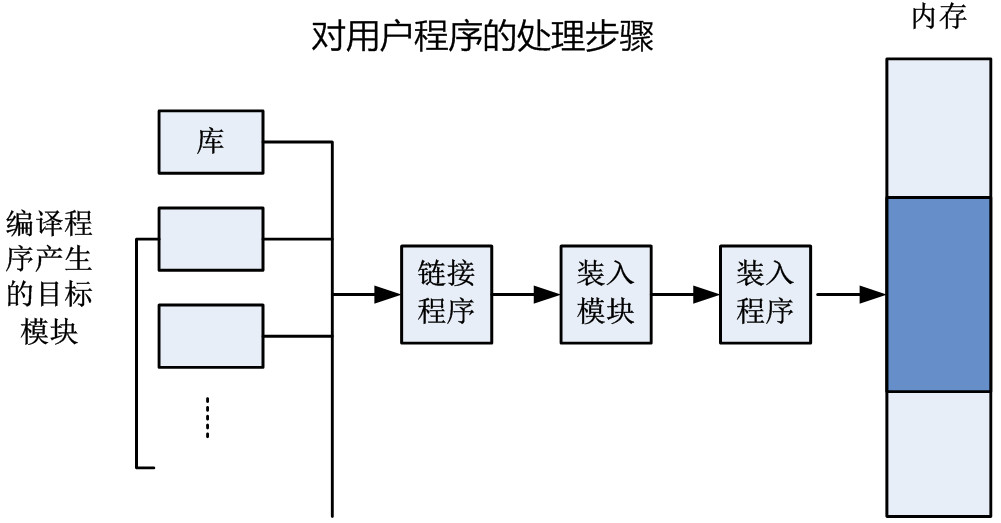
\includegraphics[width=0.9\textwidth]{figure/mem_link1.jpg}
  \end{center}
\end{frame}


\begin{frame}[fragile]{4.1.1 程序的装入 }
  \begin{easylist} 
    & 1、绝对装入(Absolute Loading Mode)
    && 编译后,装入前已产生了绝对地址(内存地址),装入时不再作地址重定位。
    && 绝对地址的产生:
    &&& (1) 由编译器完成
    &&& (2) 由程序员编程完成
    &&& 对(1)而言,编程用符号地址
    &&& 对(2)而言,要求程序员熟悉内存的使用情况,程序或数据修改后,可能要改变程序的原内存地址
  \end{easylist}
\end{frame}


\begin{frame}[fragile]{4.1.1 程序的装入 }
  \begin{easylist} 
    && 绝对装入的问题
    &&& 只能将目标模块装入到内存中事先指定的位置。在多道程序环境下,编译程序不可能预知所编译的目标模块应放在内存的何处,因此,只适用于单道程序环境。
  \end{easylist}
\end{frame}


\begin{frame}[fragile]{4.1.1 程序的装入}
  \begin{easylist} 
    & 2、可重定位装入(Relocation Loading Mode)
    && 装入时完成,主要工作是对相对地址中的指令和数据地址的调整过程,见图2
    && 地址变换通常是在装入时一次完成的,以后不再改变,故称为{\color{red}静态重定位}
    && 问题:
    &&& 不允许程序运行时在内存移动位置,但在实际运行过程中在内存中的位置要经常改变。
    &&& $\rightarrow$ 动态运行时装入方式
  \end{easylist}
\end{frame}



\begin{frame}[fragile]{作业装入内存的情况}
  \begin{center}
    \begin{tikzpicture}[c/.style={},
      a/.style={thick, -Latex}]

      \draw[thick] (0,0)--++(3,0) -- ++(0,-5)--++(-3,0)--++(0,5) ++(0,-1)--++(3,0)
      ++(0,-0.5)--++(-3,0) ++(0,-1)--++(3,0) ++(0,-0.5)--++(-3,0);

      \draw node[c] at(-0.2,0) {0} node[c] at(-0.5,-1) {1000} node[c] at(-0.5,-2.5) {2500} node[c] at(-0.5,-5) {5000} node at(1.5,-1.25) {LOAD 1, 2500};


      \draw[dotted, thick] (6,0)--++(0,1)--++(3,0)--++(0,-1);
      \draw[] (6,0)--++(3,0) -- ++(0,-5)--++(-3,0)--++(0,5) ++(0,-1)--++(3,0)
      ++(0,-0.5)--++(-3,0) ++(0,-1)--++(3,0) ++(0,-0.5)--++(-3,0);
      \draw[dotted, thick] (6,-5)--++(0,-1)--++(3,0)--++(0,1);

      \draw node[c] at(5.5,0) {10000} node[c] at(5.5,-1) {11000} node[c] at(5.5,-2.5) {12500} node[c] at(5.5,-5) {15000} node at(7.5,-1.25) {LOAD 1, 2500};
      
      \draw[thick, red!50, -Latex] (3,0)--(5,0);
      \draw[thick, red!50, -Latex] (3,-5)--(5,-5);

      \draw node at(1.5,-6) {作业地址空间} node at(7, -6) {内存空间};
    \end{tikzpicture}
  \end{center}
\end{frame}


\begin{frame}[fragile]{4.1.1 程序的装入 }
  \begin{easylist} 
    & 3.动态运行时装入
    && (Dynamic Run-time Loading)
    && 把装入模块装入内存时,并不立即把模块中的相对地址转换为绝对地址,而是推迟到程序真正要执行时才进行
    && 装入内存后的所有地址仍是相对地址
    && 一般在执行时才完成相对地址到绝对地址的转换,且有硬件的支持,能保证进程的可移动性。
  \end{easylist}
\end{frame}


\begin{frame}[fragile]{4.1.2 程序的链接}
  \begin{easylist} 
    & 1、静态链接(Static Linking)
    && a.对相对地址的修改
    && b.变换外部调用符号
    & 2、装入时动态链接(Load-time Dynamic Linking)
    && a.便于修改和更新
    && b.便于实现对目标模块的共享
    && e.g. DLL动态链接库
    & 3、运行时动态链接(Run-time Dynamic Linking)
    && e.g. Java Class Loader
  \end{easylist}
\end{frame}


\begin{frame}[fragile]{目标模块与装入模块示例}
  \begin{center}
    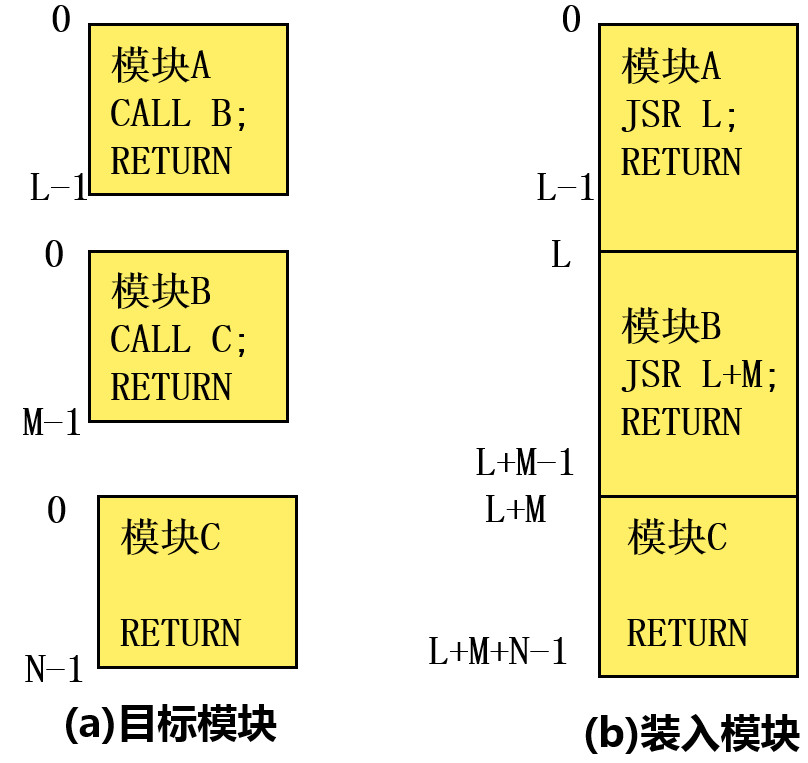
\includegraphics[width=0.6\textwidth]{figure/mem_link2.jpg}
  \end{center}
\end{frame}



\subsection{4.2 连续分配方式 }
\begin{frame}[fragile]{4.2 连续分配方式 }
  \begin{easylist} 
    & 4.2.1 单一连续分配
    && 用于单用户,单任务中
    & 4.2.2 固定分区分配
    & 4.2.3 动态分区分配
    & 4.2.4 可重定位分区分配
    & 4.2.5 对换
  \end{easylist}
\end{frame}



\begin{frame}[fragile]{4.2.1 单一连续分区}
  \begin{easylist} 
   & 最简单的存储管理方式,用于单用户、单任务OS
   & 内存划分为两部分:
   && 系统区:供OS使用,一般放在低址部分,Solaris则相反
   && 用户区
   & 存贮保护机构的设置
   && 一般不设置保护也可,因单任务运行。
   && 例如: MS-DOS, CP/M, RT-11            
  \end{easylist}
\end{frame}


\begin{frame}[fragile]{4.2.2 固定分区}
  \begin{easylist} 
  & 特点:有n个分区,则可同时装入n个作业/任务。
  & 一、分区大小:
  && 相等:
  && 不相等:不相等利用率更高。
  & 二、内存分配:
  && 数据结构: 固定分区使用表  
  &&& 将分区按大小排序,并将其地址、分配标识作记录
  & 三、特点:
  && 简单,有碎片(内零头)
  \end{easylist}
\end{frame}


\begin{frame}[fragile]{固定分区使用表}
  \begin{columns}[onlytextwidth,T]
    \begin{column}{0.5\textwidth}
      \begin{tabular}{|c|c|c|c|}
        \hline
        分区号 & 大小(k) & 起址(k) & 状态 \\ \hline
        1  & 12 & 20 & 已分配 \\ \hline
        2 & 32 & 32 & 已分配 \\ \hline
        3 & 64 & 64 & 已分配 \\ \hline
        4 & 128 & 128 & 已分配 \\ \hline
      \end{tabular}
    \end{column}

    \begin{column}{0.5\textwidth}
      \begin{tikzpicture}[c/.style={draw,thick, minimum width=2.5cm},
        tip/.style={yshift=0.2cm}]
        \small
        \draw[minimum height=1cm] node[c] (os) {操作系统}
        node[c,below=0 of os, minimum height=0.3cm, fill=yellow!60, dotted] {作业A} 
	node[c, below=0 of os, minimum height=0.8cm] (a) {}
        node[c,below=0 of a, minimum height=1cm, fill=yellow!60, dotted] {作业B} 
	node[c, below=0 of a, minimum height=1.6cm] (b) {}
        node[c,below=0 of b, minimum height=1.8cm, fill=yellow!60, dotted] {作业C} 
	node[c, below=0 of b, minimum height=2.5cm] (c) {}
        node[c, below=0 of c, minimum height=0.5cm] {$\cdots$};

        \draw[] node[below left=0 of os, tip] {20k}
        node[below left=0 of a, tip] {32k}
        node[below left=0 of b, tip] {64k}
        node[below left=0 of c, tip] {128k};
        \draw node[draw, shape=ellipse, dashed, inner sep=0cm, left=of c,minimum height=0.7cm, fill=red!15] (t) {内零头碎片};

        \path[-Latex] (t) edge (a.190) (t) edge (b.200) (t) edge (c.215);
      \end{tikzpicture}
    \end{column}
  \end{columns}
\end{frame}


\begin{frame}[fragile]{4.2.3 动态分区分配}
  \begin{easylist} 
    & 动态分区分配是根据进程的实际需要,动态为之分配内存空间。
    & 为实现动态分区分配,系统中必须配置相应的数据结构,用来描述空闲分区和已分配分区的情况。通常采用两种形式:
    && 空闲分区表
    && 空闲分区链
  \end{easylist}
\end{frame}


\begin{frame}[fragile]{一、动态分区分配的数据结构}
  \begin{easylist} 
  & 1 空闲分区表:记录每个空闲分区情况,表目包括:分区序号、分区始址及分区大小等.
  & 2 空闲分区链
  \begin{center}
    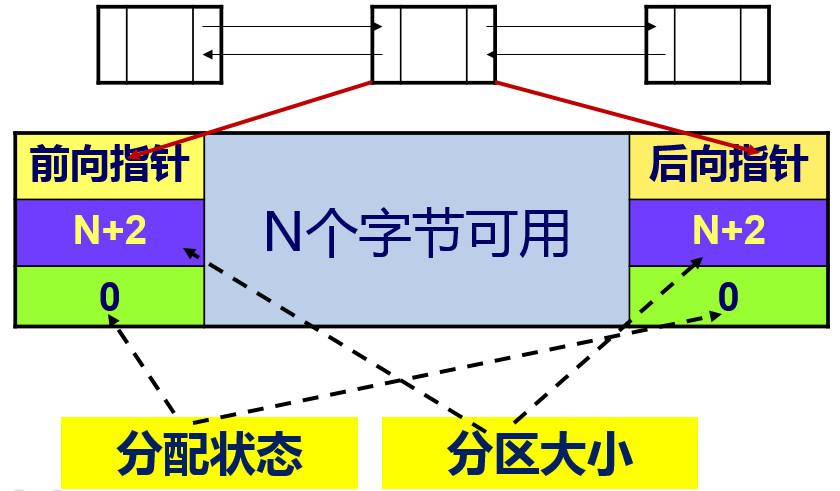
\includegraphics[width=0.6\textwidth]{figure/mem_fix1.jpg}
  \end{center}
  \end{easylist}
\end{frame}



\begin{frame}[fragile, allowframebreaks]{二、分区分配算法}
  \begin{easylist} 
    & 1 首次适应算法FF
    && 空闲区链:首址递增排列;
    && 申请:按分区的先后次序,从头查找,找到符合要求的第一个分区;
    && 优点:尽量使用低地址空间,高地址空间保持大的空闲区域。
    && 缺点:随着低地址分区不断划分而产生较多小分区(内存碎片),每次分配时查找
    时间开销会增大。

    \newpage
    & 2 循环首次适应算法
    && 空闲区链:首址递增排列;
    && 申请:从上次分配的分区起查找(到最后分区时再回到开头),找到符合要求的第一个分区,应设置一个查询指针。
    && 特点: 
    &&& 空闲分区分布均匀;
    &&& 大的空闲分区不易保留;
    &&& 查找时间开销会减小。

    \newpage
    & 3 最佳适应算法
    && 空闲区链:不是首址,而是分区容量递增排列;
    && 申请:找到符合要求的第一个分区。
    && 特点:碎片较小,但从整体来看,会形成较多的碎片。

    \newpage
    & 4 最差适应算法
    && 空闲区链:分区容量递减排列;
    && 申请:找到符合要求的第一个分区。
    && 特点:可以充分使用大的分区,但大的空闲分区不易保留。
  \end{easylist}
\end{frame}


\begin{frame}[fragile]{三、分区分配}
  \begin{easylist} 
    & 分配流程
    & 内存回收
  \end{easylist}
\end{frame}


\begin{frame}[fragile]{分配流程}
  \begin{center}
    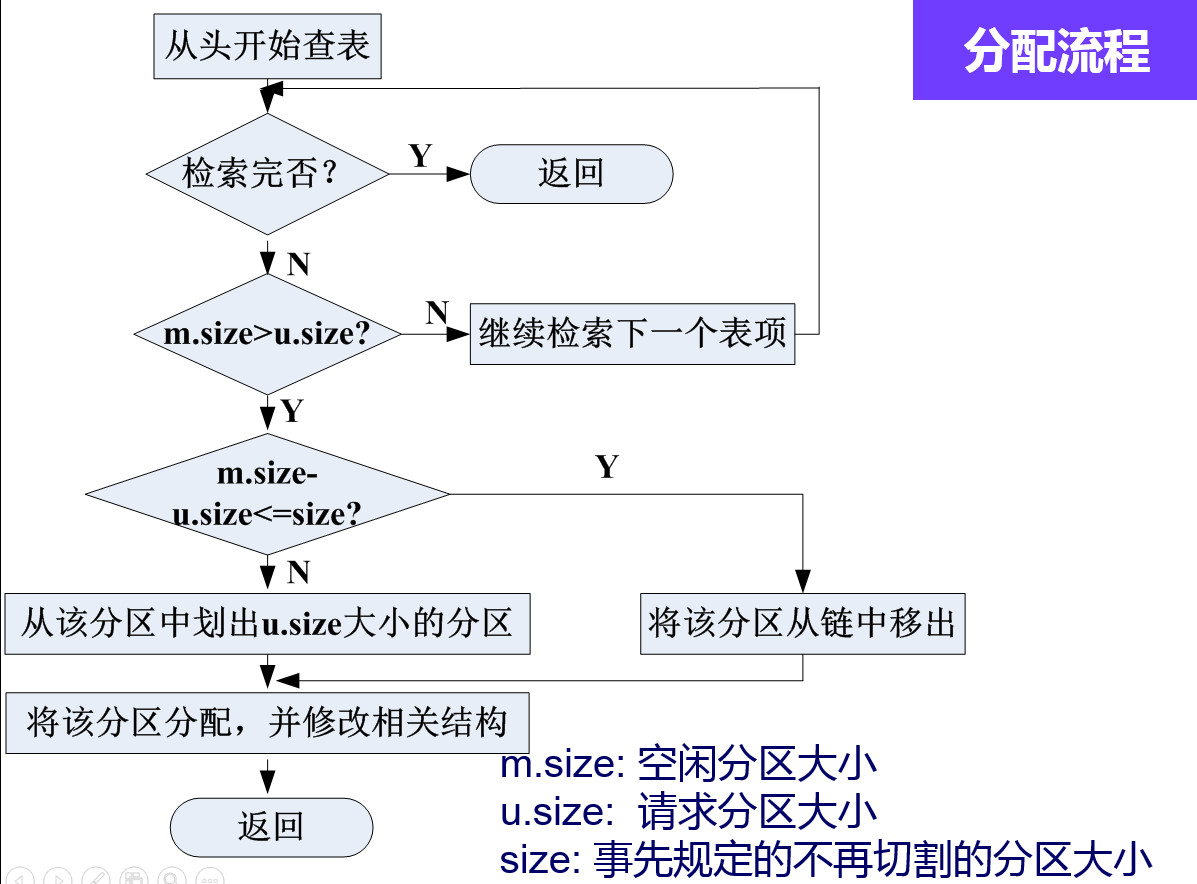
\includegraphics[width=0.8\textwidth]{figure/mem_fix2.jpg}
  \end{center}
\end{frame}


\begin{frame}[fragile]{内存回收}
  \begin{enumerate}
  \item 上邻空闲区:合并,改大小
  \item 下邻空闲区:合并,改大小,首址。
  \item 上、下邻空闲区:合并,改大小。
  \item 不邻接,则建立一新表项。
  \end{enumerate}
\end{frame}


\begin{frame}[fragile]{内存回收时的4种情况}
  \begin{center} 
    \begin{tikzpicture}[c/.style={draw,thick, minimum width=2cm, minimum height=1cm}]
      \draw[] node[c,fill=yellow!70](b1) {Free 1} 
      node[c, below=0 of b1, fill=orange!50] (b2) {回收区} 
      node[c, below=0 of b2, fill=gray!80] (b3) {Job B};
      
      \draw[] node[c,fill=yellow!70](b1) {Free 1} 
      node[c, below=0 of b1, fill=orange!50] (b2) {回收区} 
      node[c, below=0 of b2, fill=gray!80] (b3) {Job B};

      \draw[] node[c,fill=gray!80, right=of b1](b1) {Job A} 
      node[c, below=0 of b1, fill=orange!50] (b2) {回收区} 
      node[c, below=0 of b2, fill=yellow!70] (b3) {Free 2};

      \draw[] node[c,fill=yellow!70, right=of b1](b1) {Free 1} 
      node[c, below=0 of b1, fill=orange!50] (b2) {回收区} 
      node[c, below=0 of b2, fill=yellow!70] (b3) {Free 2};

      \draw[] node[c,fill=gray!80, right=of b1](b1) {Job A} 
      node[c, below=0 of b1, fill=orange!50] (b2) {回收区} 
      node[c, below=0 of b2, fill=gray!80] (b3) {Job B};
    \end{tikzpicture}
  \end{center}
\end{frame}



\begin{frame}[fragile]{课堂练习}
  \begin{easylist} 
  & 某系统采用动态分区分配方式管理内存,内存空间为640K,高端40K存放操作系统。在内
  存分配时,系统优先使用空闲区低端的空间。对下列请求序列:
  && 作业1申请130K、作业2申请60K、作业3申请100K
  && 作业2释放60K、作业4申请200K、作业3释放100K
  && 作业1释放130K、作业5申请140K、作业6申请60K
  && 作业7申请50K、作业6释放60K
  & 请分别画图表示出使用首次适应算法和最佳适应算法进行内存分配和回收后内存的实际使用情况。
  \end{easylist}
\end{frame}


\begin{frame}[fragile]{4.2.4 可重定位分区分配}
  \begin{easylist} 
  & 1 动态重定位的引入
  && 连续式分配中,总量大于作业大小的多个小分区不能容纳作业。
  && 紧凑
  &&& 通过作业移动将原来分散的小分区拼接成一个大分区。
  &&& 作业的移动需重定位。对程序和数据地址加以修改,以确保继续正常运行
  \end{easylist}
\end{frame}

\begin{frame}[fragile]{紧凑的示意}
  \begin{center}
    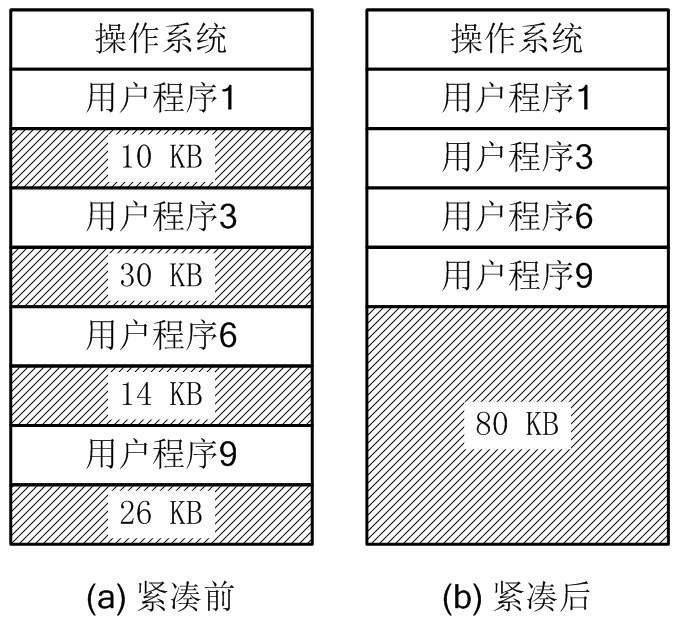
\includegraphics[width=0.6\textwidth]{figure/mem_fix_jincou.jpg}
  \end{center}
\end{frame}


\begin{frame}[fragile]{2 动态重定位的实现}
  \begin{center}
    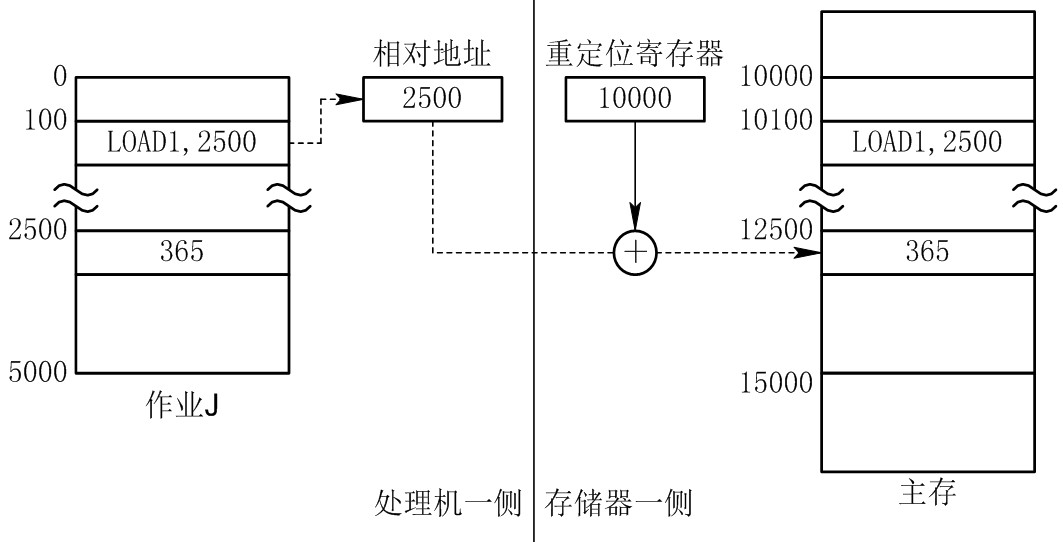
\includegraphics[width=0.9\textwidth]{figure/mem_fix_cdw.jpg}
  \end{center}
  \begin{easylist} 
   & 紧凑后,只需置换使用新起始地址即可
  \end{easylist}
\end{frame}


\begin{frame}[fragile]{动态分区分配算法流程图 }
  \begin{center}
    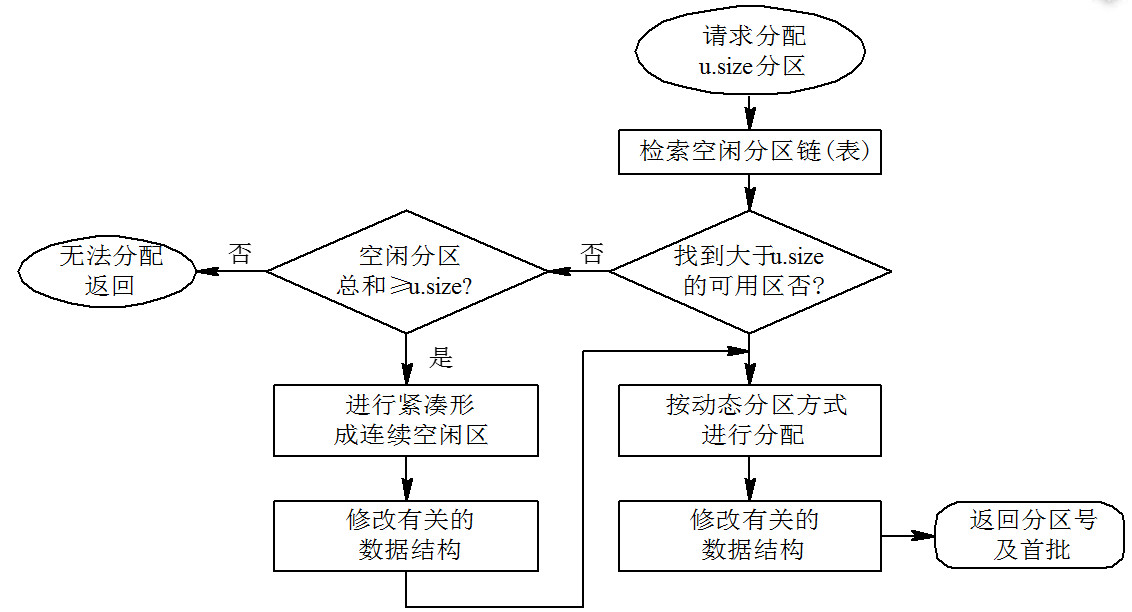
\includegraphics[width=1.0\textwidth]{figure/mem_fix_cdwlc.jpg}
  \end{center}
\end{frame}


\begin{frame}[fragile]{4.2.5 对换(Swapping)}
  \begin{easylist}
    \begin{enumerate}
      \item 对换的引入
      \item 对换空间的管理
      \item 进程的换出与换入
    \end{enumerate}
  \end{easylist}
\end{frame}


\begin{frame}[fragile]{1. 对换的引入}
  \begin{easylist} 
    & 在多道程序环境下,可以将暂时不能执行的程序送到外存中,从而获得空闲内存空间来装入新程序。
    & 所谓“对换”,是指把内存中暂时不能运行的进程或者暂时不用的程序和数据,调出
    到外存上,以便腾出足够的内存空间,再把已具备运行条件的进程或进程所需要的程序
    和数据,调入内存。对换是提高内存利用率的有效措施。
    & 如对换以整个进程为单位,称为“整体对换”或“进程对换”,广泛应用于分时系统中;
    如以“页”或“段”为单位,称为“页面对换”或“分段对换”
  \end{easylist}
\end{frame}

\begin{frame}[fragile]{对换的优缺点}
  \begin{easylist} 
   & 优点:
   && 增加并发运行的程序数目,并且给用户提供适当的响应时间;编写程序时不影响程序结构。
   & 缺点:
   && 对换入和换出的控制增加了处理机开销;
  \end{easylist}
\end{frame}


\begin{frame}[fragile]{2. 对换空间的管理}
  \begin{easylist} 
   & 把外存分为文件区和对换区。对换区用来存放从内存换出的进程。主要目标是提高进程换入和换出的速度。
   & 为了能对对换区中的空闲盘块进行管理,在系统中应配置相应的数据结构,以记录外存的使用情况。其形式与内存在动态分区分配方式中所用数据结构相似,即同样可以用空闲分区表或空闲分区链。在空闲分区表中的每个表目中应包含两项, 即对换区的首址及其大小,它们的单位是盘块号和盘块数。
  \end{easylist}
\end{frame}


\begin{frame}[fragile]{Linux下的对换空间使用情况举例}
  \begin{center}
    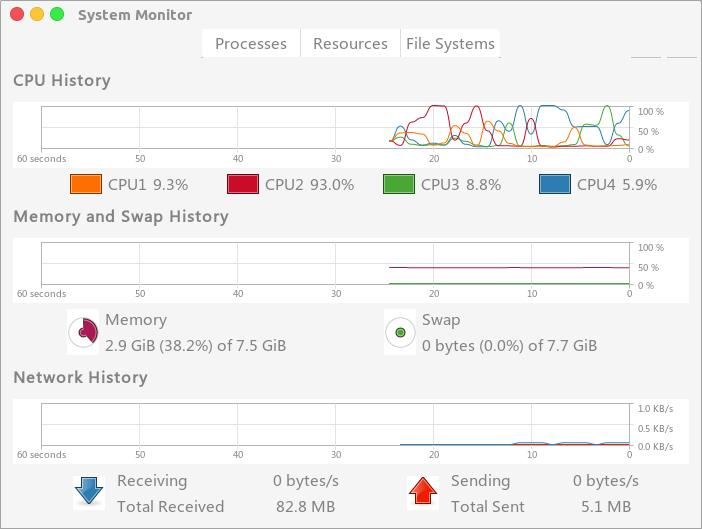
\includegraphics[width=0.8\textwidth]{figure/mem_swap_linux.jpg}
  \end{center}
\end{frame}

\begin{frame}[fragile]{Linux交换分区的大小设置建议}
  \begin{easylist} 
  & 基本原则:
  && 交换分区为内存大小的2倍
  && 交换分区不宜过大,如果内存大于2G,可以设为内存大小+2G
  && 例如:
  &&& 内存为512M,可以设为1G
  &&& 内存为4G,可以设为6G
  \vspace{1cm}
  &&& 如果内存很大的话,也可以不使用交换分区,前提是保证所有运行的程序内存总和不会超过实际内存大小
  \end{easylist}
\end{frame}


\begin{frame}[fragile]{3. 进程的换出与换入}
  \begin{easylist} 
    & 进程的换出。 
    && 每当一进程由于创建子进程而需要更多的内存空间,但又无足够的内存空间等情况发生时,系统应将某进程换出。 
    && 其过程是:系统首先选择处于阻塞状态且优先级最低的进程作为换出进程,然后启动盘块,将该进程的程序和数据传送到磁盘的对换区上。若传送过程未出现错误,便可回收该进程所占用的内存空间,并对该进程的进程控制块做相应的修改。 
    & 进程的换入
    && 系统应定时地查看所有进程的状态,从中找出“就绪”状态但已换出的进程,将其中换出时间(换出到磁盘上)最久的进程作为换入进程,将之换入,直至已无可换入的进程或无可换出的进程为止。
  \end{easylist}
\end{frame}


\begin{frame}[fragile]{PART2: 离散分配方式}
  \begin{easylist} 
  & 连续分配方式会形成许多碎片,虽然通过“紧凑”可以拼接,但是必须付出很多开销。因
  此产生了离散分配方式:
  && 分页
  && 分段
  && 段页
  \end{easylist}
\end{frame}


\subsection{4.3 基本分页存储管理方式}
\begin{frame}[fragile]{4.3 基本分页存储管理方式}
  \begin{easylist} 
   & 4.3.1 页面与页表
   & 4.3.2 地址变换机构
   & 4.3.3 两级或多级页表
  \end{easylist}
\end{frame}


\begin{frame}[fragile]{4.3.1 页面与页表 --- 页面}
  \begin{easylist} 
    & 1. 页面
    && 页面和物理块:逻辑空间和内存空间
    && 页面大小
    &&& 页太大,页内碎片大。
    &&& 页太小:页表可能很长,换入/出效率低
  \end{easylist}
\end{frame}

\begin{frame}[fragile]{页面和物理块}
  \begin{easylist} 
    & 分页存储管理,是将一个进程的逻辑地址空间分成若干个大小相等的片,称为页面或
    页,并为各页加以编号,从0开始,如第0页、第1页等。
    & 相应地,也把内存空间分成与页面相同大小的若干个存储块,称为(物理)块或页框
    (frame), 也同样为它们加以编号,如\#0、\#1等等。
    & 在为进程分配内存时,以块为单位将进程中的若干个页分别装入到多个可以不相邻接
    的物理块中。由于进程的最后一页经常装不满一块而形成了不可利用的碎片,称之为
    “页内碎片”。 
  \end{easylist}
\end{frame}


\begin{frame}[fragile]{页面大小的选择}
  \begin{easylist} 
    & 在分页系统中的页面其大小应适中。
    & 页面小:
    && 内存碎片减小,提高内存利用率
    && 每个进程占用较多页面,进程的页表过长,占用大量内存;
    && 降低页面换进换出的效率。
    & 页面大:
    && 减少页表长度,提高换进换出速度
    && 页内碎片增大
    & 页面的大小应选择应适中,且页面大小应是2的幂,通常为512B $\sim$ 8KB
  \end{easylist}
\end{frame}


\begin{frame}[fragile]{4.3.1 页面与页表 --- 地址结构}
  \begin{easylist} 
    & 2. 地址结构
    \begin{center}
      \begin{tikzpicture}[c/.style={draw,thick, minimum width=4cm, minimum height=1cm}]
	\draw[] node[c](p) {页号$P$} node[c, right=0 of p] (w) {位移量$W$};
	\draw[] node[above right=0 of w, xshift=-0.5cm] {0} node[above left=0 of w, xshift=0.7cm] {11}
        node[above right=0 of p, xshift=-0.7cm] {12} node[above left=0 of p, xshift=0.5cm] {31};
      \end{tikzpicture}
    \end{center}
   && 对某特定机器,其地址结构是一定的。若给定一个逻辑地址空间中的地址为$A$,页面
   的大小为$L$,则页号$P$和页内地址$d$可按下式求得:
   $$P=INT \left[\dfrac{A}{L} \right]$$
   $$d=[A] ~ MOD ~ L$$
   && 例: 设页大小L为1024,逻辑地址A=3186,则$P=?, d=?$
   \pause
   && Answer:$p=3, d=114$
  \end{easylist}
\end{frame}


\begin{frame}[fragile]{4.3.1 页面与页表 --- 页表}
  \begin{easylist} 
   & 3. 页表: 实现从页号到物理块号的地址映射
  \end{easylist}
  \begin{center}
    \begin{tikzpicture}[c/.style={draw,minimum height=0.5cm, minimum width=2cm},c2/.style={draw,,inner sep=0, minimum width=1.5cm,minimum height=0.5cm}]
      \draw[] node[] (up0) {用户程序};
      \foreach \x/\y in {0/0,0/1,1/2,2/3,3/4,4/5} 
      \draw[] node[c,below=0 of up\x] (up\y) {$\x$页};
      \draw[] node[c, below=0 of up5, minimum height=1cm] (up6) {$\cdots$}
      node[c, below=0 of up6] (up7) {$n$页};

      \draw[] node[right=of up0,minimum width=1.5cm] (tp0) {页号} node[right=0 of tp0,minimum width=1.5cm] (tb0) {块号};
      \draw[] node[above right=0 of tp0,xshift=-0.3cm] (tip2) {页表};
      \draw[] node[c2, below=0 of tp0] (tp0) {0}
      node[c2, below=0 of tp0] (tp1) {1} 
      node[c2, below=0 of tp1] (tp2) {2} 
      node[c2, below=0 of tp2] (tp3) {3} 
      node[c2, below=0 of tp3] (tp4) {4} 
      node[c2, below=0 of tp4] (tp5) {5} 
      node[c2, below=0 of tp5,minimum height=1cm] (tp6) {$\cdots$} ;
      \draw[] node[c2, below=0 of tb0] (tb2) {2}
      node[c2, below=0 of tb2] (tb3) {3} 
      node[c2, below=0 of tb3] (tb6) {6} 
      node[c2, below=0 of tb6] (tb8) {8} 
      node[c2, below=0 of tb8] (tb9) {9} 
      node[c2, below=0 of tb9] (tb5) {} 
      node[c2, below=0 of tb5,minimum height=1cm] (tp6) {$\cdots$} ;

      \draw[] node[right=3cm of tip2] (m0) {内存};
      \foreach \x/\y in {0/0,0/1,1/2,2/3,3/4,4/5,5/6,6/7,7/8,8/9,9/10} 
      \draw[] node[c,below=0 of m\x,minimum height=0.5cm] (m\y) {} node[right=0.1 of m\y]{$\y$};

      \path[-Latex] (tb2.east) edge (m2.west)
      (tb3.east) edge (m3.west)
      (tb6.east) edge (m6.west)
      (tb8.east) edge (m8.west)
      (tb9.east) edge (m9.west);
    \end{tikzpicture}
  \end{center}
\end{frame}


\begin{frame}[fragile]{4.3.2 地址变换机构}
  \begin{easylist} 
    & 借助于页表,实现从逻辑地址到物理地址的转换。
    & 1、基本地址变换机构:	
    && 越界保护
    && 每个进程对应一页表,其信息(如长度、始址)放在PCB中,执行时将其首地址装入页表寄存器。
  \end{easylist}
\end{frame}


\begin{frame}[fragile]{分页系统的地址变换机构}
  \begin{center}
    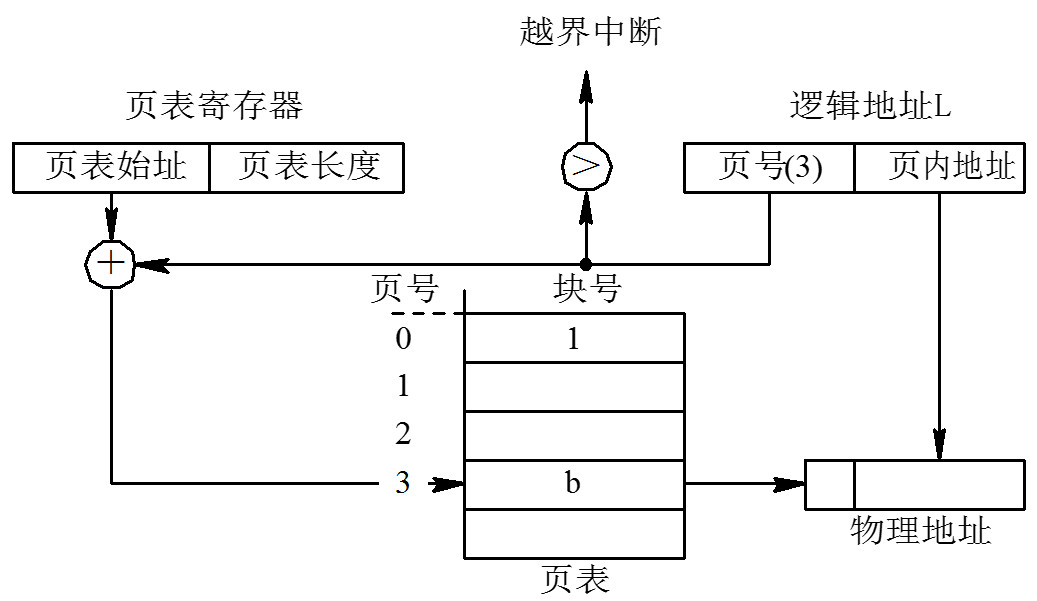
\includegraphics[width=0.9\textwidth]{figure/mem_page_dzbh.jpg}
  \end{center}
\end{frame}


\begin{frame}[fragile]{2 具有快表的地址变换机构 }
  \begin{easylist} 
    & 不具快表,则需两次访问内存。
    && (1)访页表
    && (2)得到绝对地址内容
    & 有快表,速度提高。
    & 快表贵,不能太多。
  \end{easylist}
\end{frame}


\begin{frame}[fragile]{快表}
  \begin{center}
    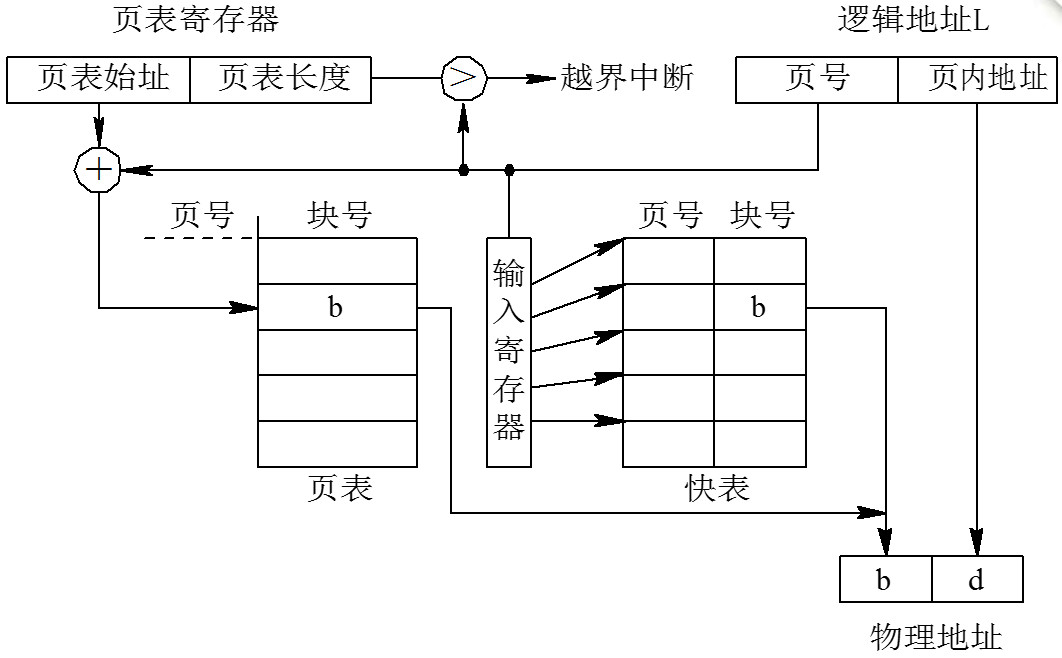
\includegraphics[width=0.9\textwidth]{figure/mem_page_cache.jpg}
  \end{center}
\end{frame}

\begin{frame}[fragile]{命中率}
  \begin{easylist} 
  & 命中率是指页号在快表中被查找到的百分比,记为$p$。则有效访问时间:
  && 访问快表的时间$\times p$ + 从内存中访问时间$\times (1-p)$
  \end{easylist}
\end{frame}


\begin{frame}[fragile]{练习}
  \begin{easylist} 
    & 有一页式系统,其页表存放在主存中:
    && 如果对主存的一次存取需要$1.5\mu s$,试问实现一次页面访问的存取时间是多少?
    && 如果系统加有快表,平均命中率为85\%,当页表项在快表中时,其查找时间忽略为0, 试问此时的存取时间是多少?
  \end{easylist}
\end{frame}

\begin{frame}[fragile]{Answer}
  \begin{easylist} 
   & 答:若页表存放在主存中,则要实现一次页面访问需两次访问主存:一次是访问页表,确定所存取页面的物理地址(称为定位)。第二次才根据该地址存取页面数据。
&& 页表在主存的存取访问时间
   $$=1.5 \times 2=3(\mu s)$$
&& 增加快表后的存取访问时间\\
  $$ =0.85 \times 1.5+(1-0.85) \times 2 \times 1.5=1.725(\mu s)$$
  \end{easylist}
\end{frame}


\begin{frame}[fragile]{练习}
  \begin{easylist} 
   & 在页式存储管理方法中,假定一页的大小为$1KB$,若一条指令在作业中的逻辑页号为
   2,页内偏移为200,该逻辑页对应的物理块的块号为7,则以四位十六进制表示的该指令
   的逻辑地址为(~~~~)H,物理地址为(~~~~)H。  \pause
   && 逻辑地址
   $$=P \times 1K+d=2×1024+200=(2248)_{10}$$
   $$ =(100011001000)_2=(08C8)_{16}$$  
   && 物理地址
   $$=f \times 1K+d=7×1024+200=(7368)_{10}$$
   $$ =(1110011001000)_2=(1CC8)_{16}$$
  \end{easylist}
\end{frame}


\begin{frame}[fragile]{4.3.3 两级和多级页表}
  \begin{easylist} 
  & 现代的大多数计算机系统,都支持非常大的逻辑地址空间($2^{32} \sim 2^{64}$)。在这样的环境下,
  页表就变得非常大,要占用相当大的内存空间。
  & 例子:
  && 对于一个具有32位逻辑地址空间的分页系统,规定页面大小为4KB即$2^{12}$B,则在
  每个进程页表中的页表项可达(~~~~)个。 
  && 每个页表项占用一个字节, 则每个进程仅其页表要占用的内存空间为(~~~~),该地址
  空间要求是(连续?|离散?)的。 \pause
  &&& 1M($\dfrac{2^{32}}{2^{12}}$)
  &&& 1M, 连续
   \end{easylist}
\end{frame}


\begin{frame}[fragile]{4.3.3 两级和多级页表}
  \begin{easylist} 
    & 解决办法:
    && 采用离散分配方式来解决难以找到一块连续的大内存空间的问题
    && 只将当前需要的部分页表项调入内存,其余的页表项仍驻留在磁盘上,需要时再调入
  \end{easylist}
\end{frame}


\begin{frame}[fragile]{1 两级页表(Two-Level Page Table)}
  \begin{easylist} 
   & 逻辑地址结构
  \end{easylist}
  \begin{center}
    \begin{tikzpicture}[]
      \coordinate (start) at (0,0);
      \draw[] node[minimum width=3cm, right=0 of start] (t1) {外层页号} node[right=0 of t1, minimum width=3cm] (t2){外层页内地址} node[right=0 of t2, minimum width=3.6cm] (t3){页内地址};
      \draw[yshift=-0.3cm, <->,blue,thick] (0,0)--(3,0);
      \draw[yshift=-0.3cm, <->,blue,thick] (3,0)--(6,0);
      \draw[yshift=-0.3cm, <->,blue,thick] (6,0)--(9.6,0);
      \draw[yshift=-1cm,thick] (0,0)--(9.6,0);
      \draw[thick] (0,-1)--(0,0.5) (3,-1)--(3,0.5) (6,-1)--(6,0.5) (9.6,-1)--(9.6,0.5);
      \draw[] node at(0,-1.5) {31} node at(2.75,-1.5) {22}  node at(3.25,-1.5) {21}
      node at(5.75,-1.5) {12}  node at(6.25,-1.5) {11}  node at(9.5,-1.5) {0};
    \end{tikzpicture}
  \end{center}
\end{frame}



\begin{frame}[fragile]{两级页表结构}
  \begin{center}
    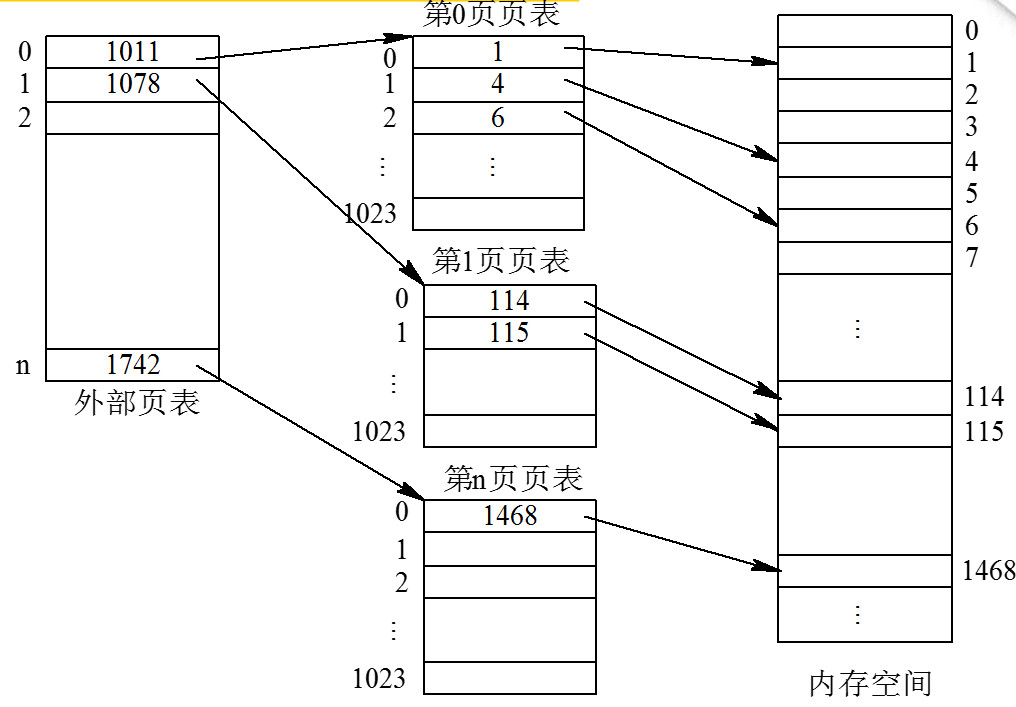
\includegraphics[width=0.9\textwidth]{figure/mem_page_ljyb.jpg}
  \end{center}
\end{frame}



\begin{frame}[fragile]{具有两级页表的地址变换机构}
  \begin{center}
    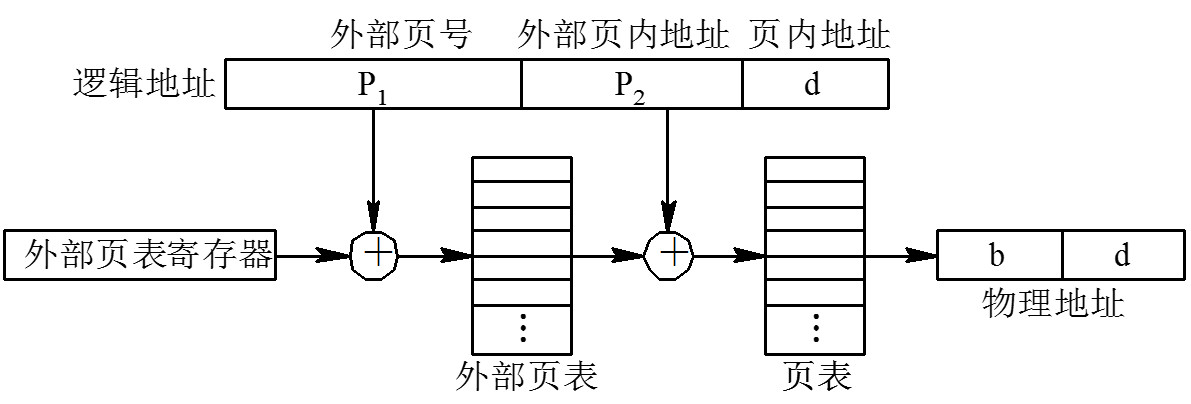
\includegraphics[width=0.9\textwidth]{figure/mem_page_ljyb2.jpg}
  \end{center}
\end{frame}


\begin{frame}[fragile]{2 多级页表}
  \begin{easylist} 
   & 对于32位的机器,采用两级页表结构是合适的;
   & 对于64位的机器,如果页面大小仍采用4KB即$2^{12}$B,即使按照两级页表划分,第
   二及页表的大小依然非常巨大
   && 引入多级页表
  \end{easylist}
\end{frame}

\begin{frame}[fragile]{NEXT}
  ~
\end{frame}


\subsection{4.4 基本分段式存储管理方式}
\begin{frame}[fragile]{4.4 基本分段式存储管理方式}
  \begin{easylist} 
    & 引入分页存储管理方式,主要是为了提高内存的利用率。而引入分段存储管理方式,主
    要是为了满足用户在编程和使用上多方面的要求。
    & 内容
    \begin{enumerate}
    \item 分段存储管理方式的引入
    \item 分段系统的基本原理
    \item 信息共享
    \item 段页式存储管理方式
    \end{enumerate}
  \end{easylist}
\end{frame}


\begin{frame}[fragile]{4.4.1分段存储管理方式的引入 }
  \begin{easylist} 
    & 引入分段存储管理方式,主要是为了满足用户和程序员的下述一系列需要:
    && 1) 方便编程
    && 2) 信息共享 
    && 3) 信息保护 
    && 4) 动态增长 
    && 5) 动态链接 
  \end{easylist}
\end{frame}



\begin{frame}[fragile]{4.4.2 分段系统的基本原理}
  \begin{easylist} 
    & 按程序自身的逻辑关系把作业的地址空间划分为若干个程序段,每个程序段都有一个
    段名,且有一个段号。段号从0开始,每一段也从0开始编址,段内地址是连续的。

  \end{easylist}
\end{frame}

\begin{frame}[fragile]{1. 分段的地址结构}
  \begin{easylist} 
  & 分段地址中的地址结构(二维的):\vspace{0.5cm}
  \begin{center}
    \begin{tikzpicture}[c/.style={draw,thick, minimum width=3cm, minimum height=0.8cm}]
      \draw[] node[c] (a) {段号} 
      node[c, right=0 of a] (b) {段内地址}
      node at (-1.5,-0.7) {31}
      node at (1.25,-0.7) {16} node at (1.75,-0.7) {15} node at (4.5,-0.7) {0} ;
    \end{tikzpicture}
  \end{center}
  & 分段方式已得到许多编译程序的支持,编译程序能自动地根据源程序的情况而产生若干
  个段。如Pascal、Fortran 
  \end{easylist}
\end{frame}

\begin{frame}[fragile]{2. 段表}
  \begin{easylist} 
  & 进程中每个分段分配一个连续的内存空间(分区),各个段可以离散地存放在内存中不
  同的分区。因此系统给每个进程建立一张映射表,简称“{\em 段表}”。{\em 段表是用于实现从逻辑段到物理内存分区的映射}。
  \end{easylist}
\end{frame}


\begin{frame}[fragile]{图:利用段表实现地址映射}
  \begin{center}
    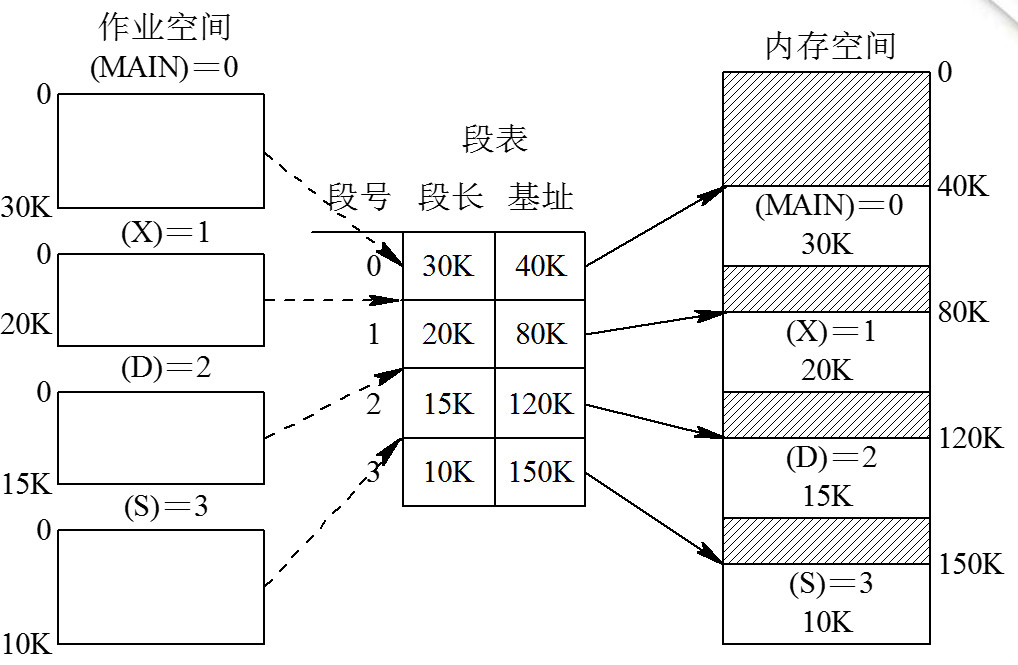
\includegraphics[width=0.8\textwidth]{figure/mem_seg1.jpg}
  \end{center}
\end{frame}

\begin{frame}[fragile]{3. 地址变换机构}
  \begin{center}
    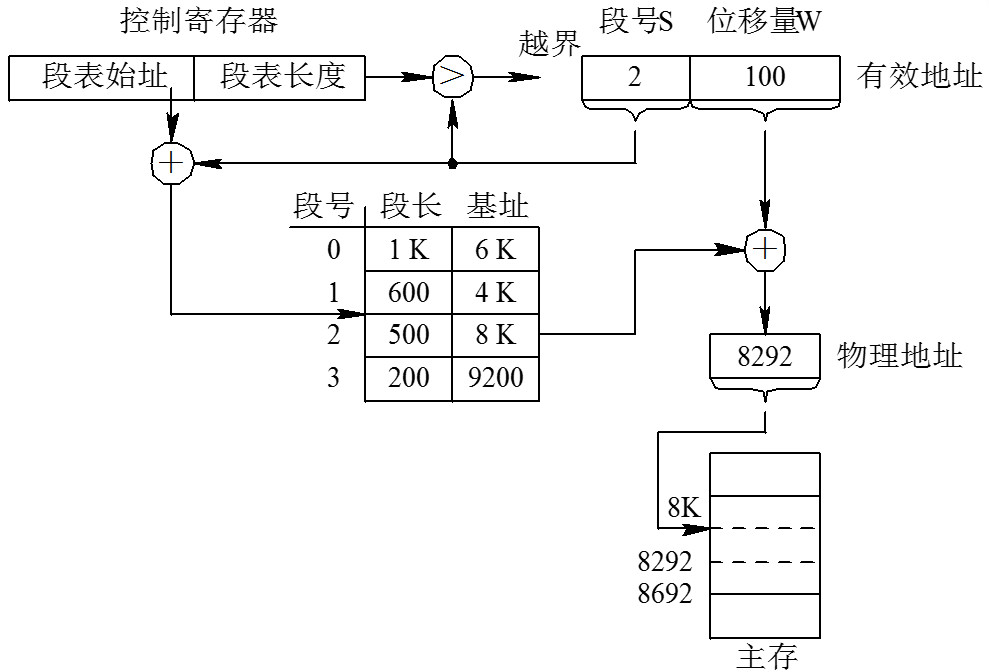
\includegraphics[width=0.8\textwidth]{figure/mem_seg2.jpg}
  \end{center}
\end{frame}

\begin{frame}[fragile]{问题}
  \begin{easylist} 
    & 要访问一个数据,需两次访问内存。同样也可以增设一个联想存储器(快表)。一般
    情况下段比页大,因而段表项的数目比页表项的数目少,其所需的联想存储器也比较小。
  \end{easylist}
\end{frame}

\begin{frame}[fragile]{4. 分页和分段的主要区别}
  \begin{easylist} 
    & [1] 页是信息的物理单位,分页是为实现离散分配方式,以消减内存的外零头, 提高
    内存的利用率。或者说, 分页仅仅是由于系统管理的需要而不是用户的需要。段则是信息
    的逻辑单位,它含有一组其意义相对完整的信息。 分段的目的是为了能更好地满足用户的
    需要。 
    & [2] 页的大小固定且由系统决定,由系统把逻辑地址划分为页号和页内地址两部分,是
    由机器硬件实现的,因而在系统中只能有一种大小的页面;而段的长度却不固定, 决定于
    用户所编写的程序,通常由编译程序在对源程序进行编译时,根据信息的性质来划分。
    & [3] 分页的作业地址空间是一维的,即单一的线性地址空间,程序员只需利用一个记忆
    符,即可表示一个地址; 而分段的作业地址空间则是二维的,程序员在标识一个地址时,
    既需给出段名,又需给出段内地址。
  \end{easylist}
\end{frame}



\begin{frame}[fragile]{4.4.3 信息共享}
  \begin{center}
    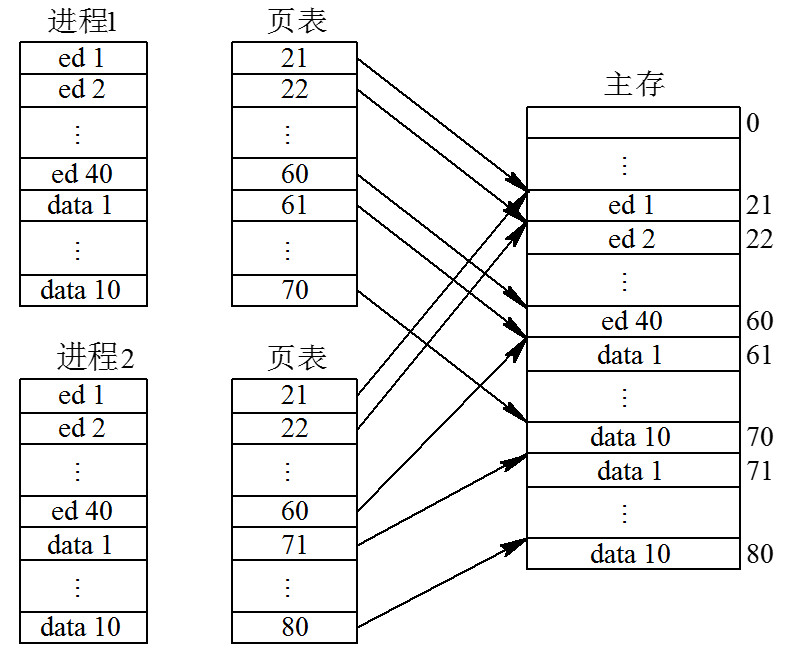
\includegraphics[width=0.7\textwidth]{figure/mem_seg3.jpg}
  \end{center}
\end{frame}


\begin{frame}[fragile]{分段系统中共享editor的示意图}
  分页系统中共享editor的示意图:
  \begin{center}
    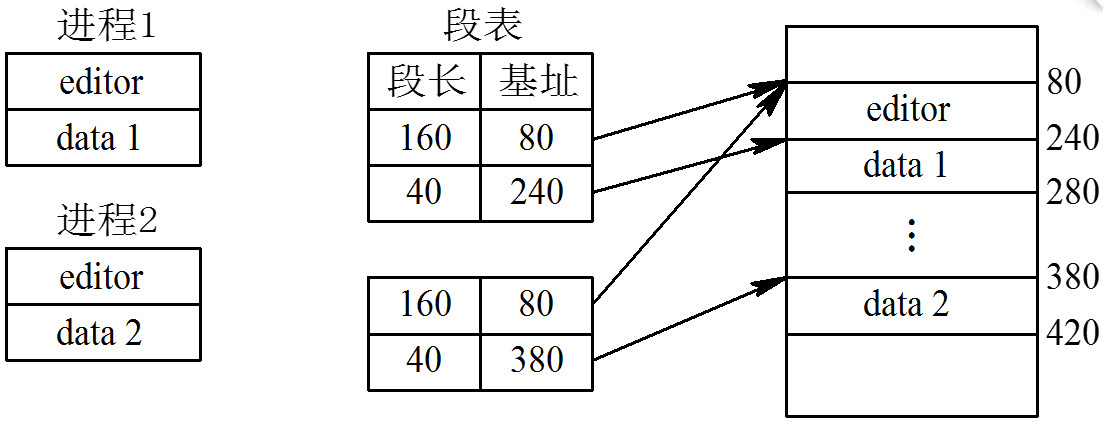
\includegraphics[width=0.8\textwidth]{figure/mem_seg4.jpg}
  \end{center}
\end{frame}


\begin{frame}[fragile]{可重入代码}
  \begin{easylist} 
    & 可重入代码又称为“纯代码”,是一种允许被多个进程同时访问的代码。
    && 为保证各个进程所执行的代码完全相同,绝对不允许可重入代码在执行中有任何改变。
    && 实际采用{\em 配备局部数据区},把执行中改变的部分拷贝到该数据区,程序执行
    只改变该进程私有的数据区,不改变共享的代码。
  \end{easylist}
\end{frame}

\begin{frame}[fragile]{4.4.4 段页式存储管理方式}
  \begin{easylist} 
    & 1 基本原理
    && 将用户程序划分若干个段,然后再把每个段分成若干页,并为每一段赋一个段名
  \end{easylist}
\end{frame}


\begin{frame}[fragile]{图: 作业地址空间和地址结构}
   \begin{center}
    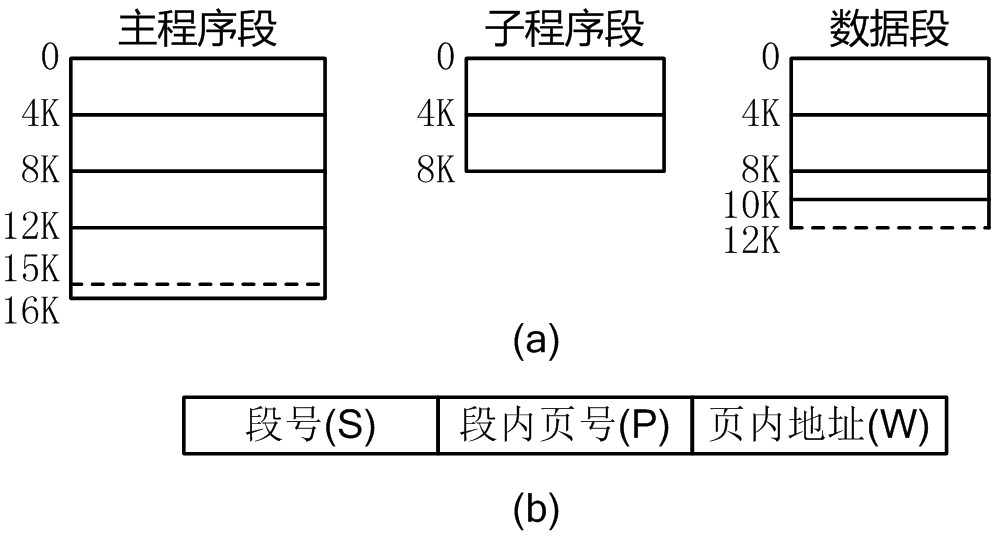
\includegraphics[width=0.8\textwidth]{figure/mem_seg5.jpg}
  \end{center}
\end{frame}


\begin{frame}[fragile]{图: 利用段表和页表实现地址映射}
 \begin{center}
    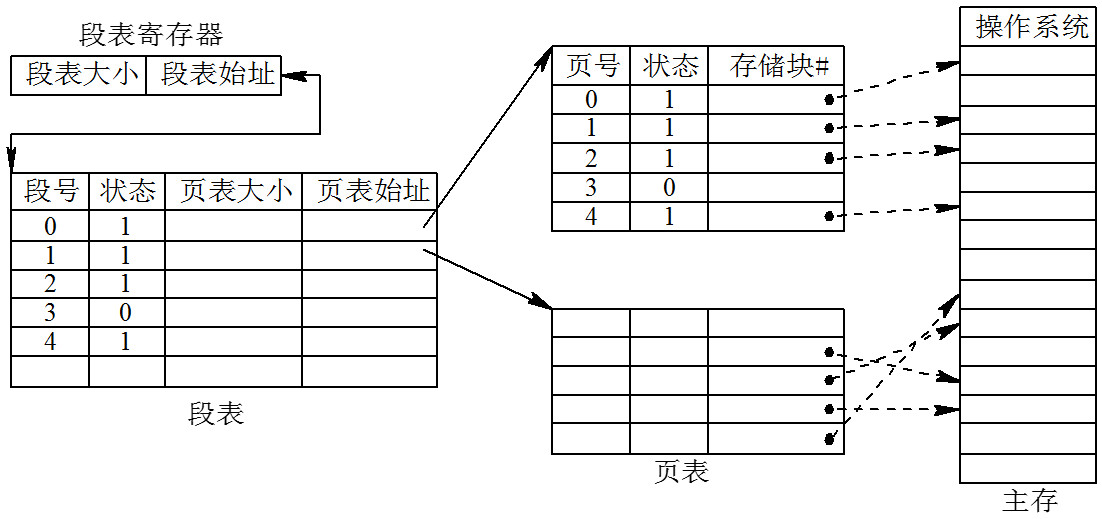
\includegraphics[width=1.0\textwidth]{figure/mem_seg6.jpg}
  \end{center}  
\end{frame}


\begin{frame}[fragile]{2 地址变换过程}
   \begin{center}
    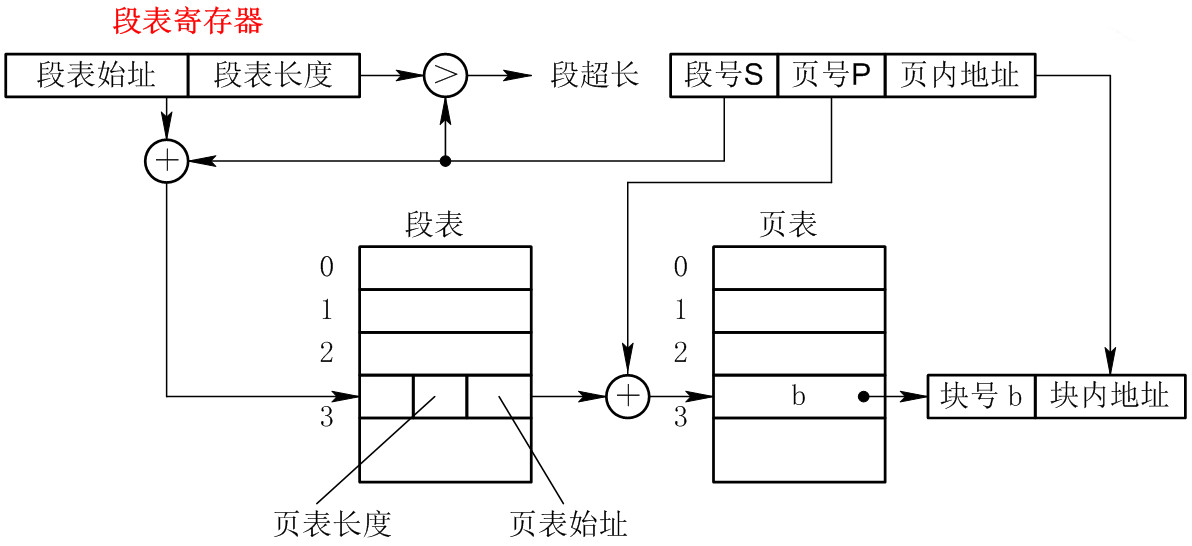
\includegraphics[width=1.0\textwidth]{figure/mem_seg7.jpg}
  \end{center}  
\end{frame}


\begin{frame}[fragile]{问题}
  \begin{easylist} 
  & 为获取一条指令或数据,需访问内存几次? \pause
  && 3次
  & 解决方法:
  && 要访问一个数据,需三次访问内存。同样也可以增设一个联想存储器(快表),存放段号和页号,访问时同时用段号和页号去检索高速缓存。
  \end{easylist}
\end{frame}

\begin{frame}[fragile]{问题}
  \begin{easylist} 
    & 连续分配方式和基本分页、分段方式的特点:要求作业全部装入内存后才能运行
    && (1) 有的作业很大,其所要求的内存空间超过了内存总容量,作业不能全部被装入
    内存,导致该作业无法运行。
    && (2) 有大量作业要求运行,但是由于内存容量不足以容纳所有这些作业,只能将少
    数的作业装入内存让它们先运行,而将其它大量的作业留在外存上等待。
    & 该怎么解决该问题?
  \end{easylist}
\end{frame}


\subsection{4.5 虚拟存储器的基本概念}
\begin{frame}[fragile]{4.5 虚拟存储器的基本概念}
  \begin{easylist} 
    & 4.5.1 虚拟存储器的引入
    & 4.5.2 虚拟存储器的实现方法
    & 4.5.3 虚拟存储器的特征
  \end{easylist}
\end{frame}

\begin{frame}[fragile]{4.5.1 虚拟存储器的引入}
  \begin{easylist} 
    & 1 常规存储器管理方式的特征
    && (1)一次性
    && (2) 驻留性
    \pause
    && 这两个特性使许多在运行中不用或暂时不用的程序/数据占据了大量的内存空间,使
    得一些需要运行的作业无法装入内存。
    && 这两个特性是否必须呢?
    &&& 程序执行的局部性
  \end{easylist}
\end{frame}

\begin{frame}[fragile]{2 局部性原理 — C++程序示例}
  \begin{center}
    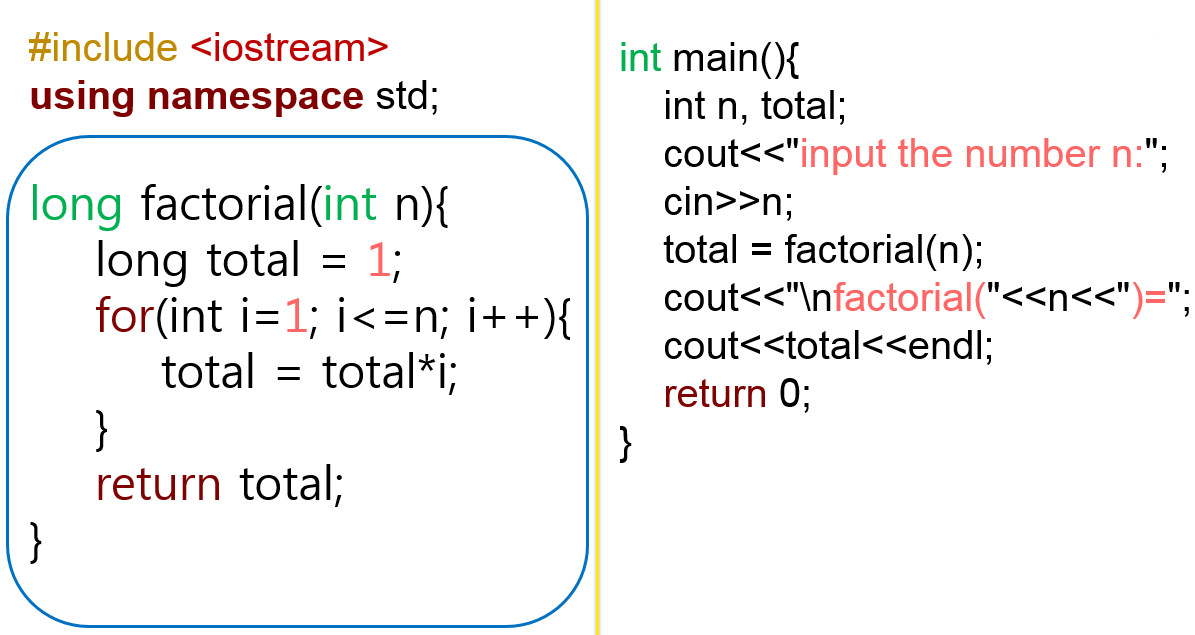
\includegraphics[width=1.0\textwidth]{figure/mem_virtual1.jpg}
  \end{center}
\end{frame}

\begin{frame}[fragile]{2 局部性原理}
  \begin{easylist} 
    & 早在1968年,Denning.P就曾指出: 
    && (1)程序执行时,除了少部分的转移和过程调用指令外,在大多数情况下仍是顺序执
    行的。
    && (2)过程调用将会使程序的执行轨迹由一部分区域转至另一部分区域,但经研究看出,
    过程调用的深度在大多数情况下都不超过5。
    && (3)程序中存在许多循环结构,这些虽然只由少数指令构成,但是它们将多次执行。
    && (4)程序中还包括许多对数据结构的处理,如对数组进行操作,它们往往都局限于很
    小的范围内。 
  \end{easylist}
\end{frame}

\begin{frame}[fragile]{局部性原理的表现方面}
  \begin{easylist} 
    & (1)时间局部性。
    && 如果程序中的某条指令一旦执行,则不久以后该指令可能再次执行;如果某数据被
    访问过, 则不久以后该数据可能再次被访问。产生时间局限性的典型原因,是由于在
    程序中存在着大量的循环操作。
    & (2)空间局部性。
    && 一旦程序访问了某个存储单元,在不久之后,其附近的存储单元也将被访问,即程
    序在一段时间内所访问的地址,可能集中在一定的范围之内,其典型情况便是程序的顺
    序执行
  \end{easylist}
\end{frame}

\begin{frame}[fragile]{3 虚拟存储器的定义}
  \begin{easylist} 
    & 虚拟存储器是指具有请求调入功能和置换功能,能从逻辑上对内存容量加以扩充的一
    种存储器系统。
    && 虚拟存储器的逻辑容量由内存容量和外存容量之和所决定,其运行速度接近于内存
    速度,而每比特的成本却又接近于外存。
    && 虚拟存储技术是一种性能非常优越的存储器管理技术,被广泛地应用于大、中、小
    型机器和微型机中。 
  \end{easylist}
\end{frame}

\begin{frame}[fragile]{4.5.2 虚拟存储器的实现方法}
  \begin{easylist} 
    & 1 分页请求系统 (以页面为单位)
    && (1)硬件支持
    &&& ①请求分页的页表机制,它是在纯分页的页表机制上增加若干项而形成的,作为请求分页的数据结构;
    &&& ②缺页中断机构,即每当用户程序要访问的页面尚未调入内存时便产生一缺页中断,以请求OS将所缺的页调入内存;
    &&& ③地址变换机构,它同样是在纯分页地址变换机构的基础上发展形成的。
    && (2)实现请求分页的软件(调页算法和置换算法)
  \end{easylist}
\end{frame}

\begin{frame}[fragile]{4.5.2 虚拟存储器的实现方法}
  \begin{easylist} 
    & 2 请求分段系统 (以段为单位)
    && (1)硬件支持
    &&& ①请求分段的段表机制,它是在纯分段的段表机制上增加若干项形成;
    &&& ②缺段中断机构,当访问尚未调入内存的分段时产生缺段中断,请求OS将所缺段调入;
    &&& ③地址变换机构。
    && (2)实现请求分段的软件(请求调段和段的置换)
  \end{easylist}
\end{frame}

\begin{frame}[fragile]{4.5.3 虚拟存储器的三个特征}
  \begin{easylist} 
    & 多次性
    && 多次性是指一个作业被分多次调入内存。多次性是虚拟存储器最重要的特征。
    & 对换性
    && 对换性是指允许在作业运行过程中换进、换出。换进和换出能够有效提高内存利用
    率。
    & 虚拟性
    && 虚拟性是指能够从逻辑上扩充内存容量,使用户所看到的内存容量远远大于实际容
    量。虚拟性是以多次性和对换性为基础的。
  \end{easylist}
\end{frame}

\begin{frame}[fragile]{Windows的虚拟内存设置}
  \begin{easylist} 
    & DEMO
  \end{easylist}
\end{frame}


\subsection{4.6 请求分页存储管理方式}
\begin{frame}[fragile]{4.6 请求分页存储管理方式}
  \begin{easylist} 
    & 建立在基本分页基础上,支持虚拟存储器功能,增加了请求调页和页面置换功能。
    && 每次调入和换出的基本单位都是长度固定的页面。
    && 比请求分段简单,是目前最常用的一种实现虚拟存储器的方式。
    \pause
    & 内容
    && 4.6.1 请求分页中的硬件支持
    && 4.6.2 内存分配策略和分配算法
    && 4.6.3 调页策略
  \end{easylist}
\end{frame}

\begin{frame}[fragile]{4.6.1 请求分页中的硬件支持}
  \begin{easylist} 
    & 1 页表机制
    & 2 缺页中断机构
    & 3 地址变换机构
  \end{easylist}
\end{frame}

\begin{frame}[fragile]{1 页表机制}
  \begin{center}
    \begin{tikzpicture}[c/.style={draw,thick, minimum width=1.5cm, minimum height=0.8cm}]
      \draw[] node[c] (a) {页号} 
      node[c, right=0 of a] (b) {物理块号}
      node[c, right=0 of b] (c) {状态位P}
      node[c, right=0 of c] (d) {访问字段A}
      node[c, right=0 of d] (e) {修改位M}
      node[c, right=0 of e] (f) {外存地址};

      \draw[draw,purple, dotted,-Latex, thick] node[c,below left=2 of c, xshift=1cm, rounded corners,fill=green!10] (g) {是否已经调入内存} (g.north)-- (c.south);

      \draw[draw, -Latex, dotted,thick, red] node[c,below left=4 of d, xshift=3cm, rounded corners,fill=green!10, align=center] (h) {被访问次数或多长时间未被访问,\\ 供选择换出页面时参考} (h.north)-- (d.south);

      \draw[draw, -Latex, dotted,thick, blue] node[c,below=2 of e,xshift=-0.5cm, rounded corners,fill=green!10] (f) {是否被修改过} (f.north)-- (e.south);
    \end{tikzpicture}
  \end{center}
\end{frame}

\begin{frame}[fragile]{2 缺页中断机构}
  \begin{easylist} 
    & 与一般中断的区别
    && 在指令执行期间产生和处理中断信号
    && 在一条指令执行期间,可能产生多次缺页中断
  \end{easylist}
\end{frame}

\begin{frame}[fragile]{图: 涉及6次缺页中断的指令}
  \begin{center}
    \begin{tikzpicture}[c/.style={draw,thick, minimum width=3cm, minimum height=0.8cm},
      c2/.style={draw,thick, minimum width=2cm, minimum height=0.5cm, red}]
      \draw[] node[c] (1) {} node[left=0.2 of 1] {1} 
      node[c, above=0 of 1] (2) {} node[left=0.2 of 2] {2}
      node[c, above=0 of 2] (3) {} node[left=0.2 of 3] {3}
      node[c, above=0 of 3] (4) {} node[left=0.2 of 4] {4}
      node[c, above=0 of 4] (5) {} node[left=0.2 of 5] {5}
      node[c, above=0 of 5] (6) {} node[left=0.2 of 6] {6} 
      node[above left=0 of 6] {页面};

      \draw[] node[c2, above=0 of 1]{copy $A$} node[c2, below=0 of 2]{to~~ $B$};
      \draw[] node[c2, above=0 of 3]{$A$ ...} node[c2, below=0 of 4]{$A$ ...};
      \draw[] node[c2, above=0 of 5]{$B$ ...} node[c2, below=0 of 6]{$B$ ...};
    \end{tikzpicture}
  \end{center}
\end{frame}

\begin{frame}[fragile]{3 地址变换机构}
  \begin{center}
    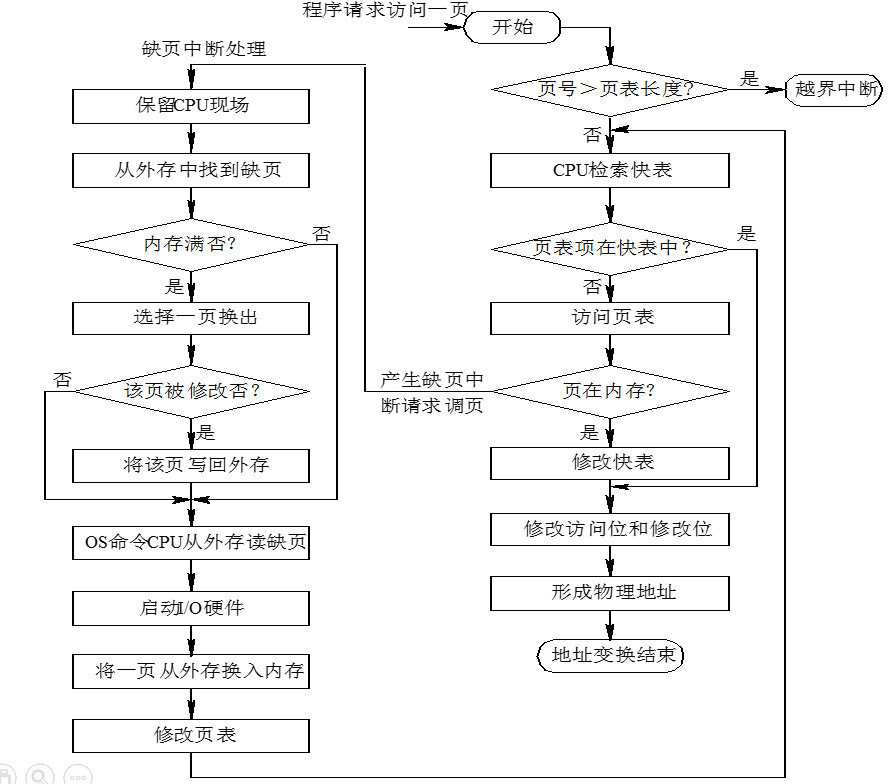
\includegraphics[width=0.8\textwidth]{figure/mem_virtual2.jpg}
  \end{center}
\end{frame}

\begin{frame}[fragile]{4.6.2 内存分配策略和分配算法}
  \begin{easylist} 
    & 1 最小物理块数的确定 
    && 最小物理块数是指能保证进程正常运行所需的最小物理块数。当系统为进程分配的
    物理块数少于此值时,进程将无法运行。
    && 最少物理块数与计算机硬件结构有关,取决于指令的格式、 功能和寻址方式。
    && 对于某些简单的机器,若是单地址指令且采用直接寻址方式,则所需的最少物理块
    数为2。
    其中,一块是用于存放指令的页面,另一块则是用于存放数据的页面。
    && 如果该机器允许间接寻址时,则至少要求有三个物理块。对于某些功能较强的机器,
    其指令长度可能是两个或多于两个字节,因而其指令本身有可能跨两个页面,且源地址
    和目标地址所涉及的区域也都可能跨两个页面。
  \end{easylist}
\end{frame}


\begin{frame}[fragile]{2 物理块的分配策略}
  \begin{easylist} 
    & 在请求分页系统中,可采取两种内存分配策略,即固定和可变分配策略。在进行置换
    时,也可采取两种策略,即全局置换和局部置换。于是可组合出以下三种适用的策略。
    && 1) 固定分配局部置换
    && 2) 可变分配全局置换 
    && 3) 可变分配局部置换
  \end{easylist}
\end{frame}

\begin{frame}[fragile]{固定分配局部置换}
  \begin{easylist} 
    & 为每个进程分配一定数目的物理块,在整个运行期间都不再改变。
    & 换出时,只能从该进程在内存的n个页面中选出一页换出,然后再调入一页,保证分
    配给该进程的内存空间不变。
    && 缺点:分配多少个物理块难以确定。
    &&& 太少,会频繁缺页,降低吞吐量;
    &&& 太多,则内存中驻留的进程数目减少,造成资源闲置。
  \end{easylist}
\end{frame}

\begin{frame}[fragile]{可变分配全局置换}
  \begin{easylist} 
    & 先为系统中的每个进程分配一定数目的物理块,OS自身也保持一个空闲物理块队列。
    缺页时,由系统从空闲物理块队列中,取出一个物理块分配给该进程。
    & 当空闲物理块用完后,OS从内存中选择任一进程的物理块调出。
  \end{easylist}
\end{frame}

\begin{frame}[fragile]{可变分配局部置换}
  \begin{easylist} 
    & 缺页时,从该进程在内存的页面中选择一页换出。(局部置换)
    & 如果频繁换页,则系统为该进程分配若干附加的物理块,直到缺页率减少到适当程度
    为止。(可变分配:增加)
    & 如缺页率特别低,则适当减少分配给该进程的物理块数。 (可变分配:减少)
  \end{easylist}
\end{frame}


\begin{frame}[fragile, allowframebreaks]{3 固定分配策略的分配算法}
  \begin{easylist} 
    & (1) 平均分配算法
    && 这是将系统中所有可供分配的物理块,平均分配给各个进程。
    && 例如,当系统中有100个物理块,有5个进程在运行时,每个进程可分得20个物理块。
    这种方式貌似公平,但实际上是不公平的,因为它未考虑到各进程本身的大小。如有一
    个进程其大小为200页,只分配给它20个块,这样,它必然会有很高的缺页率;而另一
    个进程只有10页,却有10个物理块闲置未用。
  \end{easylist}
  \newpage
  \begin{easylist} 
    & (2) 按比例分配算法
    && 这是根据进程的大小按比例分配物理块的算法。如果系统中共有$n$个进程,每个进程
    的页面数为$S_i$,则系统中各进程页面数的总和为:
    $$S=\sum_{i=1}^n S_i$$
    && 又假定系统中可用的物理块总数为$m$,则每个进程所能分到的物理块数为$b_i$,将
    有:
    $$b_i=\dfrac{S_i}{S} \cdot m$$
    &&& $b_i$应该取整,它必须大于最小物理块数。 
  \end{easylist}

  \newpage
  \begin{easylist}
    & (3) 考虑优先权的分配算法
    && 在实际应用中,为了照顾到重要的、紧迫的作业能尽快地完成,应为它分配较多的
    内存空间。
    && 通常采取的方法是把内存中可供分配的所有物理块分成两部分:
    &&& 一部分按比例地分配给各进程;
    &&& 另一部分则根据各进程的优先权,适当地增加其相应份额后,分配给各进程。在有
    的系统中,如重要的实时控制系统,则可能是完全按优先权来为各进程分配其物理块的。
  \end{easylist}
\end{frame}

\begin{frame}[fragile, allowframebreaks]{4.6.3 调页策略}
  \begin{easylist} 
    & 1 何时调入页面
    && 预调页策略
    &&& 将预计在不久之后便会访问的页面预先调入内存
    && 请求调页策略
    &&& 访问页不在内存时,立即提出请求,由OS将其调入内存。
    &&& 易于实现
    &&& 每次调入一页,开销较大
  \end{easylist}

  \newpage
  \begin{easylist}
    & 2 从何处调入页面
    && 在请求分页系统中的外存分为两部分:用于存放文件的文件区和用于存放对换页面
    的对换区。
    && 由于对换区是采用连续分配方式,而文件区是采用离散分配方式,故对换区的磁盘
    I/O速度比文件区的高。这样,每当发生缺页请求时,系统应从何处将缺页调入内存,
    可分成如下三种情况:
    \newpage
    &&& (1)系统拥有足够的对换区空间,这时可以全部从对换区调入所需页面,以提高调
    页速度。为此,在进程运行前,便须将与该进程有关的文件,从文件区拷贝到对换区。
    
    \newpage
    &&& (2)系统缺少足够的对换区空间,这时凡是不会被修改的文件,都直接从文件区调
    入;而当换出这些页面时,由于它们未被修改而不必再将它们换出,以后再调入时,仍
    从文件区直接调入。但对于那些可能被修改的部分,在将它们换出时,便须调到对换区,
    以后需要时,再从对换区调入。

    \newpage
    &&& (3)UNIX方式。由于与进程有关的文件都放在文件区,故凡是未运行过的页面,都
    应从文件区调入。而对于曾经运行过但又被换出的页面,由于是被放在对换区,因此在
    下次调入时,应从对换区调入。由于UNIX系统允许页面共享,因此, 某进程所请求的
    页面有可能已被其它进程调入内存,此时也就无须再从对换区调入。
  \end{easylist}

  \newpage
  \begin{easylist}
    & 3 页面调入过程
    && 页面未在内存时,便向CPU发出缺页中断,中断处理程序首先保留CPU环境,分析中
    断原因后, 转入缺页中断处理程序。
    && 该程序通过查找页表,得到该页在外存的物理块后, 如果此时内存能容纳新页,则
    启动磁盘I/O将所缺之页调入内存,然后修改页表。
    && 如果内存已满,则须先按照某种置换算法从内存中选出一页准备换出;如果该页未
    被修改过,就不必再写回磁盘;但如果已被修改,则必须将它写回磁盘,然后再把所缺
    的页调入内存,并修改页表中的相应表项,置其存在位为“1”,并写入快表。在缺页调
    入内存后,利用修改后的页表,去形成所要访问数据的物理地址,再去访问内存数据。
  \end{easylist}
\end{frame}


\begin{frame}[fragile]{~}
 ~
\end{frame}


\subsection{4.7 页面置换算法}
\begin{frame}[fragile]{4.7 页面置换算法}
  \begin{easylist} 
    & 页面置换算法是选择换出页面的算法。置换算法的好坏,将直接影响到系统的性能。
  \end{easylist}
\end{frame}


\begin{frame}[fragile]{4.7.1 最佳置换算法和先进先出置换算法}
  \begin{easylist} 
    & 1、最佳(Optimal)置换算法
    && 最佳置换算法是由Belady于1966年提出的一种理论上的算法。
    && 其所选择的被淘汰页面,将是以后永不使用的,或许是在最长(未来)时间内不再被
    访问的页面。
    && 采用最佳置换算法,通常可保证获得最低的缺页率。
  \end{easylist}
\end{frame}

\begin{frame}[fragile]{例}
  \begin{easylist} 
    & 假定系统为某进程分配了三个物理块, 并考虑有以下的页面号引用串:
    && 7,0,1,2,0,3,0,4,2,3,0,3,2,1,2,0,1,7,0,1
    && 进程运行时,先将7,0,1三个页面装入内存。以后,当进程要访问页面2时,将会
    产生缺页中断。此时OS根据最佳置换算法,将选择页面7予以淘汰。
  \end{easylist}
  \tiny
  \begin{center}
    \begin{tabular}{| l | c | c | c | c | c | c | c | c | c | c | c | c |c | c |c |c | c | c | c | c |}
      \hline
      \rowcolor{yellow!10}
      ~   & 7 & 0 & 1 & 2 & 0 & 3 & 0 & 4 & 2 & 3 & 0 & 3 & 2 & 1 & 2 & 0 & 1 & 7 & 0 & 1 \\
      \hline
      块1 & 7 & 7 & 7 & 2 & ~ & 2 & ~ & 2 & ~ & ~ & 2 & ~ & ~ & 2 & ~ & ~ & ~ & 7 & ~ & ~ \\ 
      块2 & ~ & 0 & 0 & 0 & ~ & 0 & ~ & 4 & ~ & ~ & 0 & ~ & ~ & 0 & ~ & ~ & ~ & 0 & ~ & ~ \\ 
      块3 & ~ & ~ & 1 & 1 & ~ & 3 & ~ & 3 & ~ & ~ & 3 & ~ & ~ & 1 & ~ & ~ & ~ & 1 & ~ & ~ \\ 
      \hline
    \end{tabular}
  \end{center}
\end{frame}

\begin{frame}[fragile]{2 先进先出(FIFO)页面置换算法}
  \tiny
  \begin{center}
    \begin{tabular}{| l | c | c | c | c | c | c | c | c | c | c | c | c |c | c |c |c | c | c | c | c |}
      \hline
      \rowcolor{yellow!10}
      ~   & 7 & 0 & 1 & 2 & 0 & 3 & 0 & 4 & 2 & 3 & 0 & 3 & 2 & 1 & 2 & 0 & 1 & 7 & 0 & 1 \\
      \hline
      块1 & 7 & 7 & 7 & 2 & ~ & 2 & 2 & 4 & 4 & 4 & 0 & ~ & ~ & 0 & 0 & ~ & ~ & 7 & 7 & 7 \\ 
      块2 & ~ & 0 & 0 & 0 & ~ & 3 & 3 & 3 & 2 & 2 & 2 & ~ & ~ & 1 & 1 & ~ & ~ & 1 & 0 & 0 \\ 
      块3 & ~ & ~ & 1 & 1 & ~ & 1 & 0 & 0 & 0 & 3 & 3 & ~ & ~ & 3 & 2 & ~ & ~ & 2 & 2 & 1 \\ 
      \hline
    \end{tabular}
  \end{center}
\end{frame}

\begin{frame}[fragile]{4.7.2 最近最久未使用(LRU)置换算法 }
  \begin{easylist} 
    & 1、LRU (Least Recently Used)置换算法的描述 
  \end{easylist}

  \tiny
  \begin{center}
    \begin{tabular}{| l | c | c | c | c | c | c | c | c | c | c | c | c |c | c |c |c | c | c | c | c |}
      \hline
      \rowcolor{yellow!10}
      ~   & 7 & 0 & 1 & 2 & 0 & 3 & 0 & 4 & 2 & 3 & 0 & 3 & 2 & 1 & 2 & 0 & 1 & 7 & 0 & 1 \\
      \hline
      块1 & 7 & 7 & 7 & 2 & ~ & 2 & ~ & 4 & 4 & 4 & 0 & ~ & ~ & 1 & ~ & 1 & ~ & 1 & ~ & ~ \\ 
      块2 & ~ & 0 & 0 & 0 & ~ & 0 & ~ & 0 & 0 & 3 & 3 & ~ & ~ & 3 & ~ & 0 & ~ & 0 & ~ & ~ \\ 
      块3 & ~ & ~ & 1 & 1 & ~ & 3 & ~ & 3 & 2 & 2 & 2 & ~ & ~ & 2 & ~ & 2 & ~ & 7 & ~ & ~ \\ 
      \hline
    \end{tabular}
  \end{center}
\end{frame}

\begin{frame}[fragile]{2、LRU算法的硬件支持}
  \begin{easylist} 
    & 1)寄存器
    && 为了记录某进程在内存中各页的使用情况,须为每个在内存中的页面配置一个移位
    寄存器,可表示为 
    $$R=R_{n-1}R_{n-2}R_{n-3} \cdots R_2 R_1 R_0$$
  \end{easylist}
\end{frame}

\begin{frame}[fragile]{图:某进程具有8个页面时的LRU访问情况}
  \begin{center}
    \begin{tabular}{| l | c | c | c | c | c | c |c |c | c | c | c | c |}
      \hline
      \rowcolor{yellow!10}
      ~   & 4 & 3 & 2 & 1 & 4 & 3 & 5 & 4 & 3 & 2 & 1 & 5  \\
      \hline
      块1 & 4 & 4 & 4 & 1 & 1 & 1 & 5 & ~ & ~ & 2 & 2 & 2 \\ 
      块2 & ~ & 3 & 3 & 3 & 4 & 4 & 4 & ~ & ~ & 4 & 1 & 1 \\ 
      块3 & ~ & ~ & 2 & 2 & 2 & 3 & 3 & ~ & ~ & 3 & 3 & 5 \\ 
      \hline
    \end{tabular}
  \end{center}
\end{frame}

\begin{frame}[fragile]{2) 栈}
  \begin{easylist} 
    & 用栈保存当前使用页面时栈的变化情况
  \end{easylist}

  \begin{center}
    \newcolumntype{g}{>{\columncolor{black!2}}c}
    \begin{tabular}{| g | c | c | c | c | c | c | c | c |}
      \hline
      \rowcolor{yellow!10}
      分页  & $R_7$ & $R_6$ & $R_5$ & $R_4$ & $R_3$ & $R_2$ & $R_1$ & $R_0$ \\
      \hline
      1 & 0 & 1 & 0 & 1 & 0 & 0 & 1 & 0 \\
      2 & 1 & 0 & 1 & 0 & 1 & 1 & 0 & 0 \\
      3 & 0 & 0 & 0 & 0 & 0 & 1 & 0 & 0 \\
      4 & 0 & 1 & 1 & 0 & 1 & 0 & 1 & 1 \\
      5 & 1 & 1 & 0 & 1 & 1 & 1 & 1 & 0 \\
      6 & 0 & 0 & 1 & 0 & 1 & 0 & 1 & 1 \\
      7 & 0 & 0 & 0 & 0 & 0 & 1 & 1 & 1 \\
      8 & 0 & 1 & 1 & 0 & 1 & 1 & 0 & 1 \\
      \hline
    \end{tabular}
  \end{center}
\end{frame}

\begin{frame}[fragile]{4.7.3 Clock置换算法}
  \begin{easylist} 
    & 1、简单的Clock置换算法 
  \end{easylist}
  \begin{center}
    \begin{tikzpicture}[b/.style={draw,minimum width=2cm, minimum height=0.6cm},
      b4/.style={draw,minimum width=1cm, minimum height=0.6cm, fill=yellow!15}]
      \draw node[b, fill=green!10](h1){块号} node[b,right=0 of h1, fill=green!10](h2){ 页号 }  node[b,right=0 of h2, fill=green!10](h3){访问位}  node[b4,right=0 of h3, fill=green!10](h4){指针} ;
      \draw node[b, below=0 of h1](b01){0} node[b,right=0 of b01](b02){ }  node[b,right=0 of b02](b03){ }  node[b4,right=0 of b03](b04){ } ;
      \draw node[b, below=0 of b01](b11){1} node[b,right=0 of b11](b12){ }  node[b,right=0 of b12](b13){ }  node[b4,right=0 of b13](b14){ } ;
      \draw node[b, below=0 of b11](b21){2} node[b,right=0 of b21](b22){4 }  node[b,right=0 of b22](b23){0 }  node[b4,right=0 of b23](b24){ } ;
      \draw node[b, below=0 of b21](b31){3} node[b,right=0 of b31](b32){ }  node[b,right=0 of b32](b33){ }  node[b4,right=0 of b33](b34){ } ;
      \draw node[b, below=0 of b31](b41){4} node[b,right=0 of b41](b42){2 }  node[b,right=0 of b42](b43){1 }  node[b4,right=0 of b43](b44){ } ;
      \draw node[b, below=0 of b41](b51){5} node[b,right=0 of b51](b52){ }  node[b,right=0 of b52](b53){ }  node[b4,right=0 of b53](b54){ } ;
      \draw node[b, below=0 of b51](b61){6} node[b,right=0 of b61](b62){5 }  node[b,right=0 of b62](b63){ 0}  node[b4,right=0 of b63](b64){ } ;
      \draw node[b, below=0 of b61](b71){7} node[b,right=0 of b71](b72){ 1}  node[b,right=0 of b72](b73){1 }  node[b4,right=0 of b73](b74){ } ;

      \draw node[right=of b24, yshift=0.15cm](p){替换指针};
      \draw[-latex, thick] (p) -- +(-2.3,0);

      \draw[-latex, thick] (b24.345) --+(-0.3,0) -- ++(1,0) -- ++(0,-1) -- ++(-1.5,0);
      \draw[-latex, thick] (b44.345) --+(-0.3,0) -- ++(1,0) -- ++(0,-1) -- ++(-1.5,0);
      \draw[-latex, thick] (b64.345) --+(-0.3,0) -- ++(1,0) -- ++(0,-0.5) -- ++(-1.5,0);
    \end{tikzpicture}
  \end{center}
\end{frame}

\begin{frame}[fragile]{2 改进的Clock置换算法}
  \begin{easylist}
    & 由访问位A和修改位M可以组合成下面四种类型的页面:
    && 1类(A=0, M=0):表示该页最近既未被访问,又未被修改,是最佳淘汰页。
    && 2类(A=0, M=1):表示该页最近未被访问, 但已被修改,并不是很好的淘汰页。
    && 3类(A=1, M=0):最近已被访问,但未被修改,该页有可能再被访问。
    && 4类(A=1, M=1):最近已被访问且被修改, 该页可能再被访问。
  \end{easylist}
\end{frame}


\begin{frame}[fragile]{执行过程}
  \begin{easylist}
    & (1)从指针所指示的当前位置开始,扫描循环队列,寻找A=0且M=0的第一类页面,将
    所遇到的第一个页面作为所选中的淘汰页。在第一次扫描期间不改变访问位A。
    & (2)如果第一步失败,即查找一周后未遇到第一类页面,则开始第二轮扫描,寻找A=0
    且M=1的第二类页面,将所遇到的第一个这类页面作为淘汰页。在第二轮扫描期间,将
    所有扫描过的页面的访问位都置0。
    & (3)如果第二步也失败,亦即未找到第二类页面,则将指针返回到开始的位置,并将
    所有的访问位复0。然后重复第一步,如果仍失败,必要时再重复第二步,此时就一定
    能找到被淘汰的页。 
  \end{easylist}
\end{frame}

\begin{frame}[fragile]{4.7.4 其他置换算法}
  \begin{easylist}
    & 最少使用置换算法
    && (LFU:Least Frequently Used)
    & 页面缓冲算法
    && (PBA:Page Buffering Algorithm) 
  \end{easylist}
\end{frame}

\begin{frame}[fragile]{练习}
  \begin{easylist}
& 在一个请求分页存储管理系统中,一个作业的页面走向为4、3、2、1、4、3、5、4、3、2、1、5,当分配给该作业的物理块数分别为3、4时,试计算采用下述页面算法时的缺页次数(假设开始执行时主存中没有页面),并比较所得结果。
&& (1) 最佳置换法(OPT)
&& (2) 先进先出法(FIFO)
  \end{easylist}
\end{frame}

\begin{frame}[fragile]{解:OPT,物理块为3时}
  (1) 根据所给页面走向,使用最佳置换算法时,页面置换情况如下:
  
  \begin{center}
    \begin{tabular}{| l | c | c | c | c | c | c | c | c | c | c | c | c |}
      \hline
      \rowcolor{yellow!10}
      ~   & 4 & 3 & 2 & 1 & 4 & 3 & 5 & 4 & 3 & 2 & 1 & 5 \\
      \hline
      块1 & 4 & 4 & 4 & 4 & ~ & ~ & 4 & ~ & ~ & 2 & 2 & ~ \\ 
      块2 & ~ & 3 & 3 & 3 & ~ & ~ & 3 & ~ & ~ & 3 & 1 & ~ \\ 
      块3 & ~ & ~ & 2 & 1 & ~ & ~ & 5 & ~ & ~ & 5 & 5 & ~ \\
      \hline
    \end{tabular}
  \end{center}

  因此,缺页次数为7;
\end{frame}

\begin{frame}[fragile]{解:OPT,物理块为4时}
  \begin{center}
    \begin{tabular}{| l | c | c | c | c | c | c | c | c | c | c | c | c |}
      \hline
      \rowcolor{yellow!10}
      ~   & 4 & 3 & 2 & 1 & 4 & 3 & 5 & 4 & 3 & 2 & 1 & 5 \\
      \hline
      块1 & 4 & 4 & 4 & 4 & ~ & ~ & 4 & ~ & ~ & ~ & 1 & ~ \\ 
      块2 & ~ & 3 & 3 & 3 & ~ & ~ & 3 & ~ & ~ & ~ & 3 & ~ \\ 
      块3 & ~ & ~ & 2 & 2 & ~ & ~ & 2 & ~ & ~ & ~ & 2 & ~ \\
      块4 & ~ & ~ & ~ & 1 & ~ & ~ & 5 & ~ & ~ & ~ & 5 & ~ \\
      \hline
    \end{tabular}
  \end{center}

  \begin{easylist}
    & 因此,缺页次数为6。
    & 由上述结果可以看出,增加分配给作业的内存块数可以降低缺页次数。
  \end{easylist}
\end{frame}

\begin{frame}[fragile]{解:FIFO,物理块为3时}
  (2) 根据所给页面走向,使用先进先出页面置换算法时,页面置换情况如下:
    % \includegraphics[width=0.9\textwidth]{figure/mem_replace8.jpg}

  \begin{center}
    \begin{tabular}{| l | c | c | c | c | c | c | c | c | c | c | c | c |}
      \hline
      \rowcolor{yellow!10}
      ~   & 4 & 3 & 2 & 1 & 4 & 3 & 5 & 4 & 3 & 2 & 1 & 5 \\
      \hline
      块1 & 4 & 4 & 4 & 1 & 1 & 1 & 5 & ~ & ~ & 5 & 5 & ~ \\ 
      块2 & ~ & 3 & 3 & 3 & 4 & 4 & 4 & ~ & ~ & 2 & 2 & ~ \\ 
      块3 & ~ & ~ & 2 & 2 & 2 & 3 & 3 & ~ & ~ & 3 & 1 & ~ \\
      \hline
    \end{tabular}
  \end{center}

  因此,缺页次数为9;
\end{frame}


\begin{frame}[fragile]{解:FIFO,物理块为4时}
  \begin{center}
    \begin{tabular}{| l | c | c | c | c | c | c | c | c | c | c | c | c |}
      \hline
      \rowcolor{yellow!10}
      ~   & 4 & 3 & 2 & 1 & 4 & 3 & 5 & 4 & 3 & 2 & 1 & 5 \\
      \hline
      块1 & 4 & 4 & 4 & 4 & ~ & ~ & 5 & 5 & 5 & 5 & 1 & 1 \\ 
      块2 & ~ & 3 & 3 & 3 & ~ & ~ & 3 & 4 & 4 & 4 & 4 & 5 \\ 
      块3 & ~ & ~ & 2 & 2 & ~ & ~ & 2 & 2 & 3 & 3 & 3 & 3 \\
      块4 & ~ & ~ & ~ & 1 & ~ & ~ & 1 & 1 & 1 & 2 & 2 & 2 \\
      \hline
    \end{tabular}
  \end{center}

  \begin{easylist}
    & 因此,缺页次数为10;
    & 由上述结果可以看出,对先进先出算法而言,增加分配给作业的内存块数反而出现缺页次数增加的异常现象。
  \end{easylist}
\end{frame}


\subsection{4.8 请求分段存储管理方式}
\begin{frame}[fragile]{4.8 请求分段存储管理方式}
  略...
\end{frame}


\begin{frame}[fragile]{练习}
  \begin{easylist} \easyitem
    & 简述逻辑地址和物理地址
    & 固定分区、可变分区和页式存储管理各有什么样的优缺点
    & 分页管理中为什么需要页表?简述其作用。
    & 简述利用请求分页实现虚拟存储器的基本原理
  \end{easylist}
\end{frame}

\begin{frame}[fragile]{实验}
  \begin{easylist}
    & 实现LRU算法和FIFO算法
    & 要求
    && 给出任意的输入流、计算缺页率。
    && 输入流长度、分配的物理块$B$的大小可定制。
    && 例如:
    &&& $B=5$, 逻辑页为0-9个数字的任意排序,输入流的长度为30。
    &&& 输入流:1 2 5 6 8 3 6 5 3 6 5 6 8 9 2 7 0 4 9 5 3 6 7 4 5 8 7 3 4 5
  \end{easylist}
\end{frame}

\begin{frame}
  \begin{center}
    \Huge END
  \end{center}
\end{frame}

%%% Local Variables:
%%% mode: latex
%%% TeX-master: "../os"
%%% End:
